\thispagestyle{thachthuctoanhocnone}
\pagestyle{thachthuctoanhoc}
\everymath{\color{thachthuctoanhoc}}
\graphicspath{{../thachthuctoanhoc/pic/}}
\begingroup
\AddToShipoutPicture*{\put(0,616){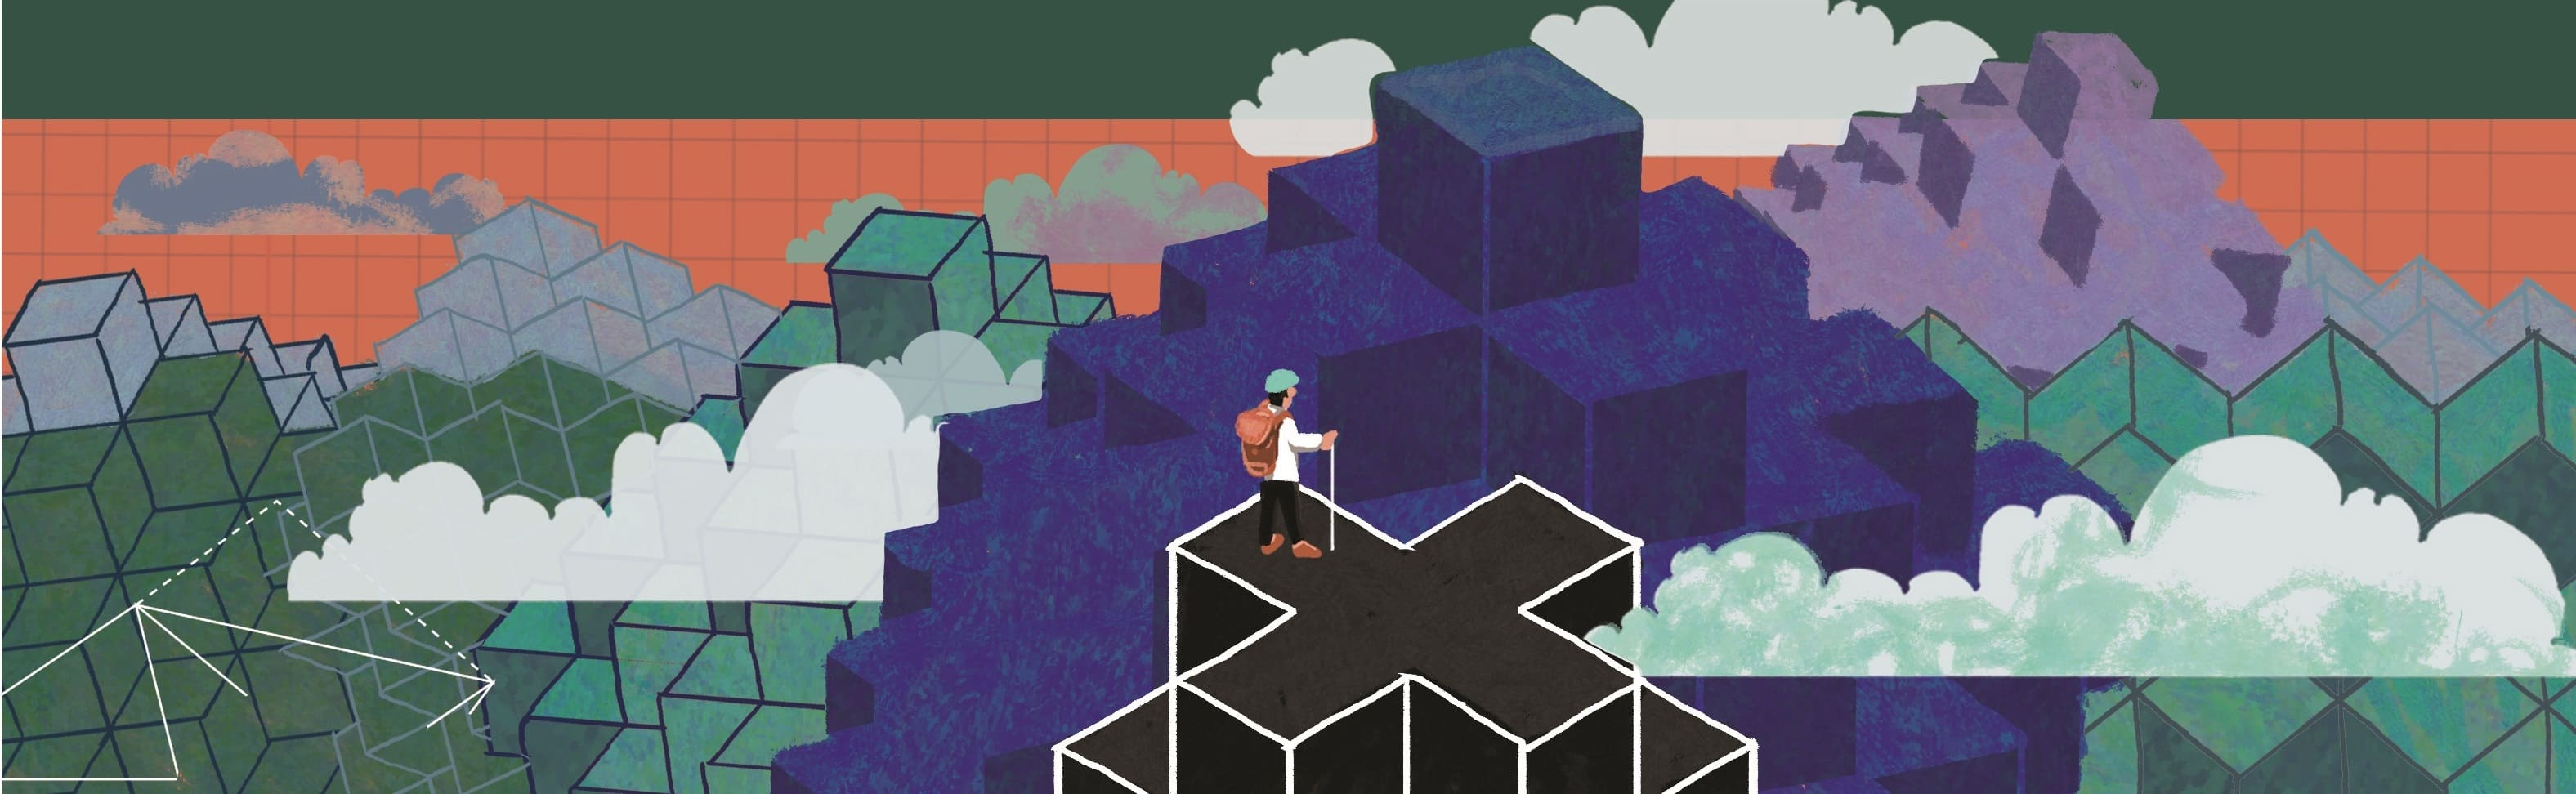
\includegraphics[width=19.3cm]{../thachthuctoanhoc/bannerthachthuc}}}
\centering
\vspace*{4cm}
\endgroup
\vspace*{-8pt}
\begin{tBox}
	\begin{itemize}[leftmargin = 13pt, itemsep = 1.0pt] 
		%		\item Mỗi bài toán đề xuất (kèm theo lời giải) cần được nêu rõ là bài sáng tác hay bài sưu tầm.
		\item Mỗi bài toán đề xuất (kèm theo lời giải) cần được nêu rõ là bài sáng tác hay bài sưu tầm (nếu là bài sưu tầm, cần ghi rõ nguồn).
		\item Bài giải cho mỗi bài toán cần được trình bày trong một file riêng hoặc
		một tờ giấy riêng.
		\item  Người đề xuất bài toán hoặc gửi bài giải cho các bài toán trong mục ``Thách thức kỳ này" cần ghi rõ họ, đệm, tên và nơi làm việc/học tập, số điện thoại liên hệ. Nếu là học sinh (hoặc sinh viên) cần ghi rõ là học sinh lớp mấy (hoặc sinh viên năm thứ mấy).
		\item Các bài toán trong mục Thách thức kỳ này hướng tới các độc giả là học sinh phổ thông; được phân chia thành các mức độ $B$, $A$, và được sắp xếp theo độ khó tăng dần, theo đánh giá chủ quan của Ban biên tập. Các bài toán mức độ $B$ không đòi hỏi các kiến thức vượt quá chương trình môn Toán cấp THCS; các bài toán mức độ $A$ không đòi hỏi các kiến thức vượt quá chương trình môn Toán cấp THPT.
		\item Cách thức gửi bài toán đề xuất hoặc lời giải: gửi file thu được bằng cách scan, ảnh chụp (rõ nét) của bản viết tay, hoặc được soạn thảo bằng các phần mềm Latex, Word tới \url{bbt@pi.edu.vn} hoặc gửi qua đường bưu điện tới Tòa soạn (xem địa chỉ tại bìa $2$).
		\item Hạn gửi lời giải cho các bài toán P$611$--P$620$: trước ngày $15/8/2022$.
	\end{itemize}
\end{tBox}
\begin{center}
	\vspace*{-5pt}
	\textbf{\color{thachthuctoanhoc}THÁCH THỨC KỲ NÀY}
	\vspace*{-5pt}
\end{center}
\begin{multicols}{2}
	\setlength{\abovedisplayskip}{4pt}
	\setlength{\belowdisplayskip}{4pt}
	{\color{thachthuctoanhoc}{\usefont{T5}{qag}{b}{n} P611.}}
	(Mức $B$) Cho $A,B,C$ là các chữ số khác $0$ sao cho $\overline{CCA}+\overline{B2B}=\overline{A88}$. Hãy tìm số $\overline{ABC}$. 
	\vskip 0.05cm
	\hfill	\textit{Tường Thanh, Nghệ An (st)}
	\vskip 0.05cm
	{\color{thachthuctoanhoc}{\usefont{T5}{qag}{b}{n} P612.}}
	(Mức $B$) Chứng minh biểu thức sau nhận giá trị nguyên với mọi giá trị nguyên dương của $n$
	\begin{align*}
		A\!=\!\dfrac{\left(2^4\!+\!\dfrac14\right)\!\left(4^4\!+\!\dfrac14\right)\!\cdots\! \left((2n)^4\!+\!\dfrac14\right)}{\left(1^4\!+\!\dfrac14\right)\left(3^4\!+\!\dfrac14\right)\!\cdots\! \left((2n\!-\!1)^4\!+\!\dfrac14\right)}.
	\end{align*}
	\vskip 0.05cm
	\hfill	\textit{Phùng Chí Tự, Hà Nội (st)}
	\vskip 0.05cm
	{\color{thachthuctoanhoc}{\usefont{T5}{qag}{b}{n} P613.}}
	(Mức $B$) Cho $n$ là một số nguyên dương. Chứng minh rằng, trong ba số $n$,  $\dfrac{n-5}2$, và $\dfrac{15n-9}7$, có ít nhất hai số không phải là số chính phương.
	\begin{flushright}
		\textit{Trương Quang An, Quảng Ngãi}
	\end{flushright}
	{\color{thachthuctoanhoc}{\usefont{T5}{qag}{b}{n} P614.}}
	(Mức $B$) Cho $a,b$ là các số nguyên dương thoả mãn
	\begin{align*}
		\left\{ \sqrt{a+\sqrt{a}}\right\}=\{\sqrt b\}.
	\end{align*}
	Chứng minh rằng, $4b+1$ là một số chính phương.
	\vskip 0.05cm
	(Với $x$ là một số thực, $\{x\}=x-[x]$, trong đó $[x]$ là số nguyên lớn nhất không vượt quá $x$. Đại lượng $\{x\}$ được gọi là {\it phần lẻ} của số thực $x$)
	\begin{flushright}
		\textit{Lưu Bá Thắng, Hà Nội}
	\end{flushright}
	{\color{thachthuctoanhoc}{\usefont{T5}{qag}{b}{n} P615.}}
	(Mức $B$) Cho tam giác $ABC$ vuông tại $A$. Một điểm $D$ di chuyển trên tia $CA$. Gọi $E$ là hình chiếu vuông góc của điểm $C$ trên đường thẳng $BD$; $F$ là giao điểm của $AE$ và $BC$. Chứng minh rằng, đường thẳng $DF$ luôn đi qua một điểm cố định.
	\begin{figure}[H]
		\vspace*{-5pt}
		\centering
		\captionsetup{labelformat= empty, justification=centering}
		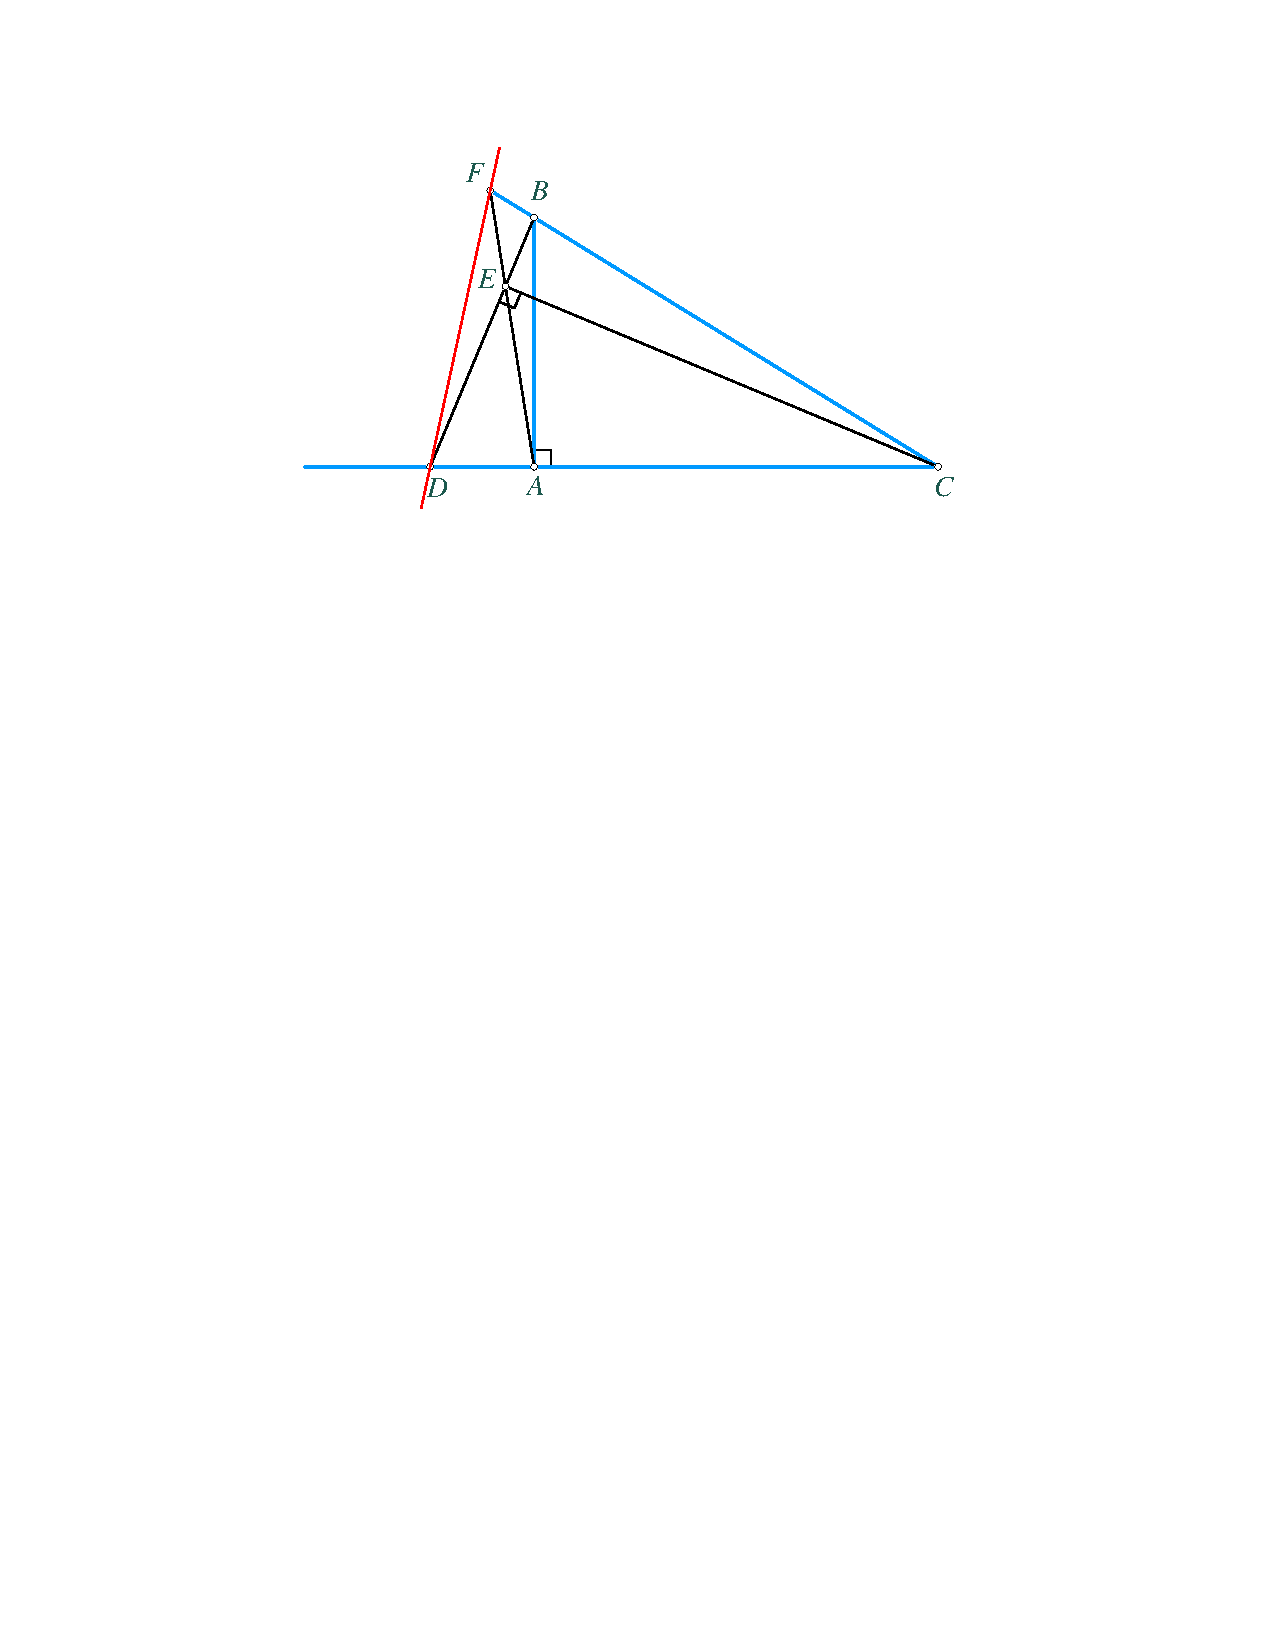
\includegraphics[width= 1\linewidth]{P615}
		\vspace*{-15pt}
	\end{figure}
	\hfill	\textit{Trần Thanh Hưng, Phú Yên}
	\vskip 0.05cm
	{\color{thachthuctoanhoc}{\usefont{T5}{qag}{b}{n} P616.}}
	(Mức $B$) Xét các số dương $a,b,c$ thoả mãn $a+b+c=4$. Tìm giá trị nhỏ nhất của biểu thức 
	\begin{align*}
		P=\left|\dfrac 1a-1\right|+\left|\dfrac 1b-1\right|+\left|\dfrac 1c-1\right|.
	\end{align*}
	\begin{flushright}
		\textit{Nguyễn Tuấn Ngọc, Tiền Giang}
	\end{flushright}
	{\color{thachthuctoanhoc}{\usefont{T5}{qag}{b}{n} P617.}}
	(Mức $A$) Giải phương trình
	\begin{align*}
		\sqrt{(x^3-4)^3}=\sqrt[3]{(x^2+4)^2}+4.
	\end{align*} 
	\begin{flushright}
		\textit{Trần Văn Lâm, Thái Nguyên (st)}
	\end{flushright}
	{\color{thachthuctoanhoc}{\usefont{T5}{qag}{b}{n} P618.}}
	(Mức $A$) Cho $a,b,c$ là các số nguyên lớn hơn $1$. Giả sử $x,y,z$ là các số thực thoả mãn $a^x=bc$, $b^y=ca$ và $c^z=ab$. Tính giá trị của biểu thức $T=x+y+z-xyz$. 
	\vskip 0.05cm
		\hfill \textit{Bằng Linh, Phú Thọ (st)}
	\vskip 0.05cm
	\columnbreak
	{\color{thachthuctoanhoc}{\usefont{T5}{qag}{b}{n} P619.}}
	(Mức $A$) Cho tam giác $ABC$ nội tiếp đường tròn $(O)$, có trực tâm $H$. Gọi $M$ là điểm chính giữa cung $BAC$ của $(O)$. Qua $O$ kẻ đường thẳng  song song với $AM$, cắt $HM$ tại $P$. Gọi $X,Y,Z$ tương ứng là hình chiếu vuông góc của $P$ trên $BC,CA,AB$. Chứng minh rằng đường tròn ngoại tiếp tam giác $XYZ$ đi qua trung điểm của $HM.$
	\begin{figure}[H]
		\vspace*{-10pt}
		\centering
		\captionsetup{labelformat= empty, justification=centering}
		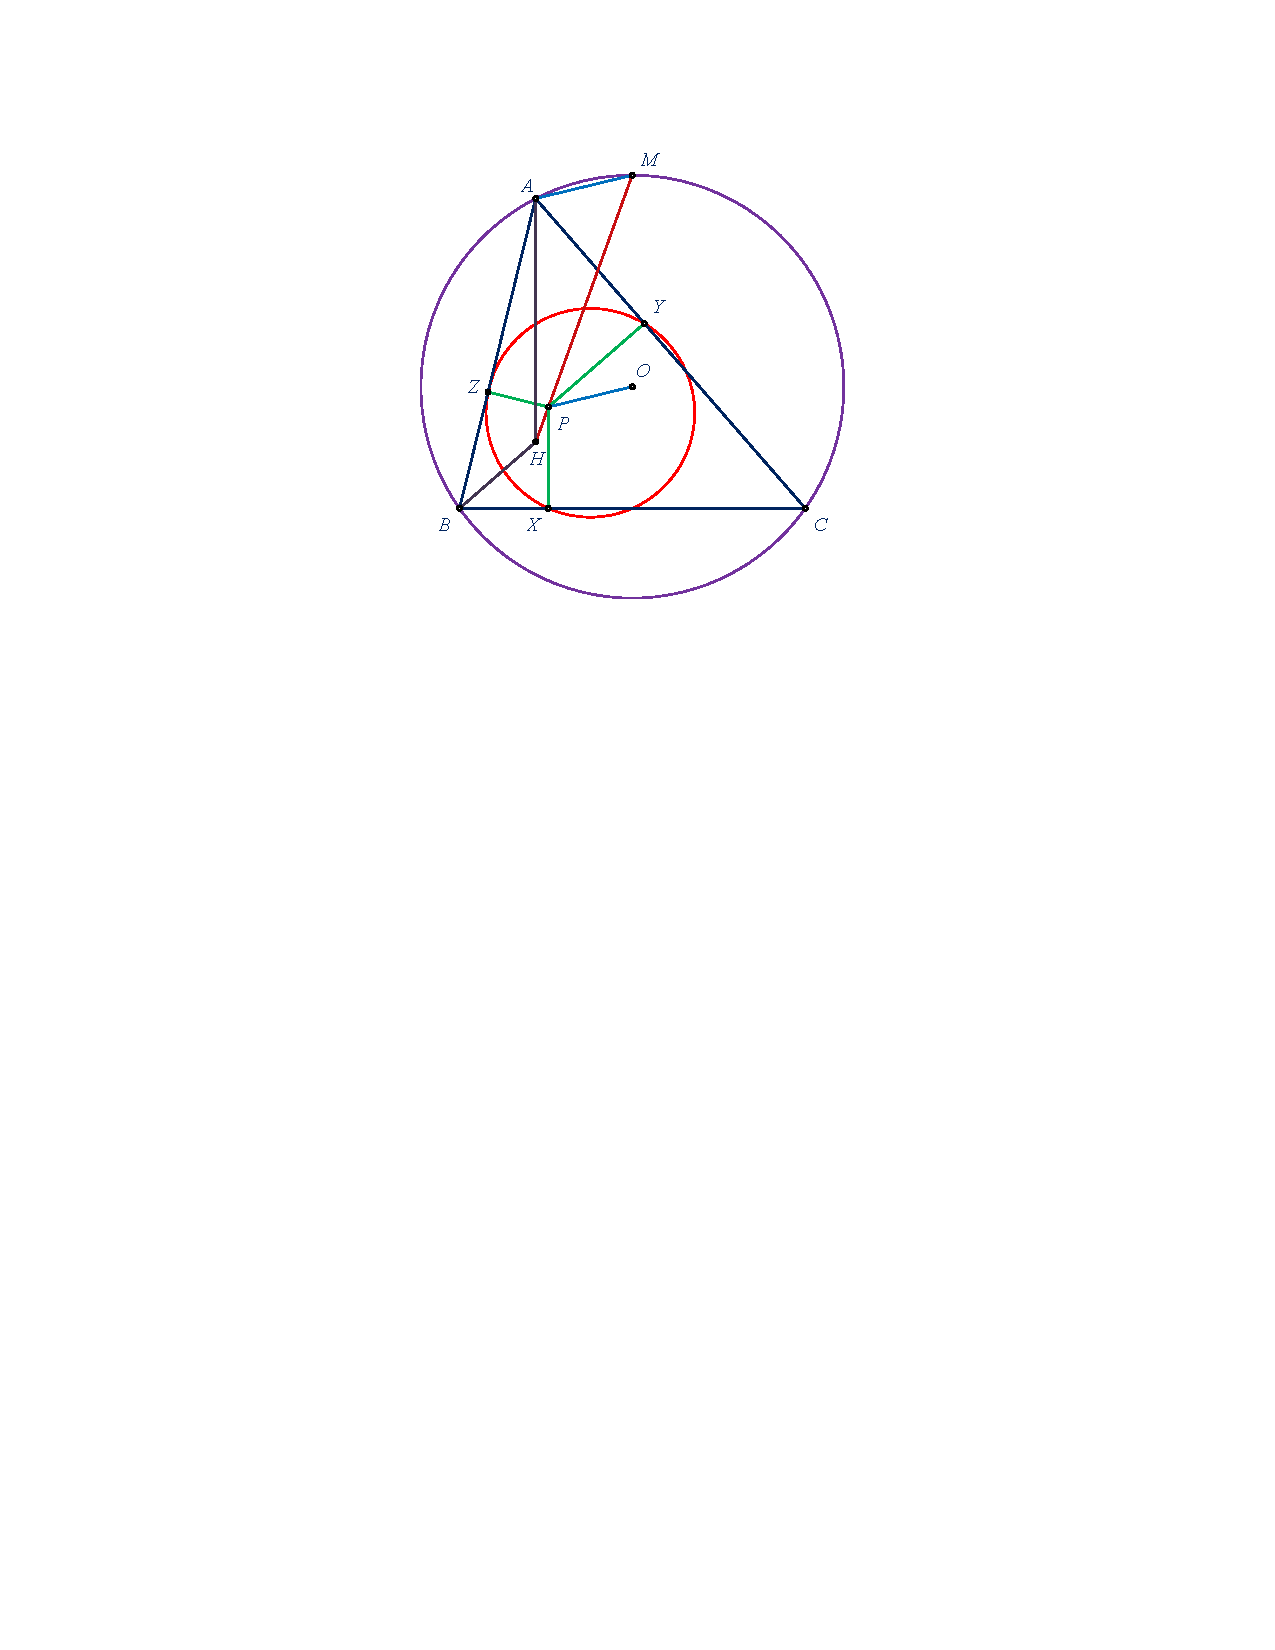
\includegraphics[width= 1\linewidth]{P619}
		\vspace*{-15pt}
	\end{figure}
	\begin{flushright}
		\textit{Nguyễn Văn Linh, Hà Nội}
	\end{flushright}
	{\color{thachthuctoanhoc}{\usefont{T5}{qag}{b}{n} P620.}}
	(Mức $A$) Chứng minh rằng với mọi số nguyên tố $p\ge5$, tồn tại số nguyên $t$ sao cho: với mọi số nguyên $k$ thì $k^2-2t^2-1$ không chia hết cho $p$.   
	\begin{flushright}
		\textit{Nguyễn Quang Minh, Singapore}
	\end{flushright}
\end{multicols}
\begin{center}
	{\large{\textbf{\color{thachthuctoanhoc}\color{thachthuctoanhoc}GIẢI BÀI KỲ TRƯỚC}}}
\end{center}
\begin{multicols}{2}
	\setlength{\abovedisplayskip}{4pt}
	\setlength{\belowdisplayskip}{4pt}
	{\color{thachthuctoanhoc}{\usefont{T5}{qag}{b}{n} P581.}}
	(Mức $B$) Xét năm số nguyên khác nhau $a, b, c, d, e$, sao cho tổng của ba số bất kỳ trong chúng lớn hơn tổng của hai số còn lại. Tìm giá trị nhỏ nhất của tổng
	\begin{align*}
		S = abcd + abce + abde + acde + bcde.
	\end{align*}
	\textbf{\color{thachthuctoanhoc}Lời giải} (\textit{phỏng theo ý tưởng giải của tất cả các bạn đã gửi lời giải tới Tạp chí})\textbf{\color{thachthuctoanhoc}.}
	\vskip 0.05cm
	Do vai trò của năm số $a, b, c, d, e$ trong bài toán là như nhau, nên không mất tính tổng quát, giả sử
	\begin{align*}
		a > b > c > d > e.\tag{$1$}
	\end{align*}                                                             
	Khi đó, do các số nêu trên là các số nguyên nên
	\begin{align*}
		a - c \ge 2 \text{\color{black} \,và } b - d \ge 2. \tag{$2$}
	\end{align*}
	Theo giả thiết, ta có:
	\begin{align*}
		c+d+e > a+b;
	\end{align*}
	do đó \hspace*{25pt}$e >  (a - c) + (b - d).$ \hfill ($3$)
	\end{multicols}
	\begin{multicols}{2}
	\setlength{\abovedisplayskip}{4pt}
	\setlength{\belowdisplayskip}{4pt}
	Từ ($2$) và ($3$), suy ra $e\ge 4$. Vì thế, từ ($1$), với lưu ý $a, b, c, d$ là các số nguyên, ta được: $d\ge 5$, $c\ge 6$, $b\ge 7$ và $a\ge 8$. Do đó
	\begin{align*}
		S &\ge 8 \cdot 7 \cdot 6 \cdot 5 + 8 \cdot 7 \cdot 6 \cdot 4 + 8 \cdot 7 \cdot 5 \cdot 4 \\
		&+ 8 \cdot 6 \cdot 5 \cdot 4 + 7 \cdot 6 \cdot 5 \cdot 4 = 11274.
	\end{align*}
	Dấu bằng đạt được khi $a= 8, b= 7,$ \linebreak$c= 6, d= 5$ và $e= 4$.
	\vskip 0.05cm
	Hơn nữa, dễ thấy, bộ năm số nguyên vừa nêu trên thỏa mãn tất cả các yêu cầu của đề bài.
	\vskip 0.05cm
	Vì vậy, giá trị nhỏ nhất của tổng $S$ bằng $11274$.
	\vskip 0.05cm
	\textbf{\color{thachthuctoanhoc}Bình luận và Nhận xét}
	\vskip 0.05cm
	Rất tiếc, tuy tất cả các lời giải Tạp chí nhận được đều có ý giải đúng và có đáp số đúng, nhưng không được coi là lời giải hoàn chỉnh, do người giải bài không đề cập việc kiểm tra bộ năm số nguyên, mà ứng với nó, $S$ nhận giá trị $11274$, có thỏa mãn các yêu cầu của đề bài hay không.
	\begin{flushright}
		\textbf{\color{thachthuctoanhoc}Lê Huy}
	\end{flushright}
	{\color{thachthuctoanhoc}{\usefont{T5}{qag}{b}{n} P582.}}
	(Mức $B$) Bạn Tâm nghĩ trong đầu một số nguyên lớn hơn $2$ và nhỏ hơn $26$. Bạn An hỏi bạn Tâm ba câu hỏi sau về số mà bạn Tâm nghĩ:
	\vskip 0.05cm
	-- Số đó có phải là số chính phương không?
	\vskip 0.05cm
	-- Số đó có phải là số nguyên tố không?
	\vskip 0.05cm
	-- Số đó có chia hết cho $n$ không?,
	\vskip 0.05cm
	trong đó $n$ là một số tự nhiên chẵn có một chữ số, do An tự chọn.
	\vskip 0.05cm
	Biết rằng, căn cứ câu trả lời của Tâm cho ba câu hỏi trên, An đã đoán được chính xác số Tâm nghĩ trong đầu. Hỏi, An đã chọn số n nào, và số Tâm nghĩ là số nào?
	\vskip 0.05cm
	\textbf{\color{thachthuctoanhoc}Lời giải} (\textit{của người chấm bài})\textbf{\color{thachthuctoanhoc}.}
	\vskip 0.05cm
	Gọi $k$ là số Tâm nghĩ trong đầu;theo giả thiết, $k \in \mathbb{Z}$  và $2 <k< 26$.
	\vskip 0.05cm
	Ký hiệu $S$ là tập hợp các số nguyên lớn hơn $2$ và nhỏ hơn $26$; và ký hiệu $S_1, S_2, S_3$  tương ứng là tập hợp các số chính phương thuộc $S$, tập hợp các số nguyên tố thuộc $S$, tập hợp các số đồng thời không chính phương, không nguyên tố thuộc $S$. Ta có:
	\begin{align*}
		&{S_1}\, = \left\{ {4;9;16;25} \right\}\\
		&{S_2}\, = \left\{ {3;5;7;11;13;17;19;23} \right\},\\
		&{S_3}\, = \left\{ {6;8;10;12;14;15;18;20;21;22;24} \right\}.
	\end{align*}
	Rõ ràng, $k$ thuộc đúng một trong ba tập  $S_1, S_2, S_3$.
	\vskip 0.05cm
	Dễ thấy, các câu trả lời cho hai câu hỏi đầu tiên (theo thứ tự liệt kê trong đề bài) giúp An xác định chính xác $k$ thuộc tập nào trong ba tập  $S_1, S_2, S_3$, và câu trả lời cho câu hỏi thứ ba giúp An có đúng một phương án cho việc đoán số $k$.
	\vskip 0.05cm
	Vì thế, từ định nghĩa số $n$ và giả thiết ``An đoán chính xác số $k$", suy ra, tập  \linebreak$S_i (i \in \{1; 2; 3\})$ chứa $k$ là tập, mà có thể chọn được số $n \in \{2; 4; 6; 8\}$, sao cho trong tập ấy có duy nhất số có tính chất ``chia hết cho $n$", hoặc có tính chất ``không chia hết cho $n$", và $k$ chính là số duy nhất này.
	\vskip 0.05cm
	Nhận thấy, với mọi $n \in \{2; 4; 6; 8\}$, tất cả các số thuộc tập $S_2$  đều không chia hết cho $n$, và trong tập $S_3$  luôn có ít nhất hai số chia hết cho $n$, cũng như luôn có ít nhất hai số không chia hết cho $n$. Vì thế, $k \notin S_2$  và  $k \notin S_3$. Suy ra, $k \in S_1$.
	\vskip 0.05cm 
	Với $n= 2$, hoặc $n= 4$, trong tập  $S_1$ luôn có đúng hai số chia hết cho $n$, và có đúng hai số không chia hết cho $n$.
	\vskip 0.05cm
	Với $n= 6$, cả bốn số thuộc  $S_1$ cùng không chia hết cho $n$.
	\vskip 0.05cm
	Với $n= 8$, trong tập $S_1$  có duy nhất số $16$ chia hết cho $n$,và ba số còn lại không chia hết cho~$n$.
	\vskip 0.05cm
	Từ ba nhận xét vừa nêu trên, hiển nhiên suy ra, số $n$ An chọn là $8$, và số Tâm nghĩ trong đầu là $16$.
	\vskip 0.05cm
	\textbf{\color{thachthuctoanhoc}Bình luận và Nhận xét}
	\vskip 0.05cm
	$\pmb{1.}$ Ngoài cách suy diễn đã nêu trong lời giải trên, còn có thể tìm ra câu trả lời cho câu hỏi của bài toán nhờ các cách suy diễn khác; ví dụ, thông qua việc xét các khả năng có thể xảy ra đối với bộ ba câu trả lời cho bộ ba câu hỏi đã nêu trong đề bài.
	\vskip 0.05cm
	$\pmb{2.}$ Trong số các lời giải Tạp chí đã nhận được từ bạn đọc, có một số lời giải đã mắc những sai sót rất đáng tiếc trong quá trình lập luận. Chẳng hạn, có bạn đã lập luận sai rằng, ``với $n= 2$, trong tập hợp $\{6; 8; 10; 12; 14; 15; 18; 20; 21; 22; 24\}$ có duy nhất số $15$ không chia hết cho $2$"; hay có bạn đã lập luận sai rằng, ``nếu số Tâm nghĩ trong đầu là số nguyên tố thì với $n$ là số tự nhiên chẵn có một chữ số, cả ba câu hỏi đã nêu trong đề bài đều có câu trả lời là ``không";~\ldots 
	\vskip 0.05cm
	$\pmb{3.}$ Cùng với các lời giải mắc lỗi nêu trên, có một lời giải khác không được chấp nhận là lời giải hoàn chỉnh, do các lập luận trong lời giải đó thiếu chặt chẽ, và thiếu các chứng minh cần thiết cho những khẳng định mang tính then chốt được nêu ra.
	\begin{flushright}
		\textbf{\color{thachthuctoanhoc}Hà Thanh}
	\end{flushright}
	{\color{thachthuctoanhoc}{\usefont{T5}{qag}{b}{n} P583.}}
	(Mức $B$) Giả sử $a, b$ là các số dương, sao cho $a + b + \frac{1}{a} + \frac{1}{b}$ và  ${a^3}\, + {b^3}\, + \frac{1}{{{a^3}}} + \frac{1}{{{b^3}}}$ đều là các số hữu tỷ. Chứng minh rằng
	\begin{align*}
		{a^2}\, + {b^2}\, + \frac{1}{{{a^2}}} + \frac{1}{{{b^2}}}
	\end{align*}
	cũng là một số hữu tỷ.
	\vskip 0.05cm
	\textbf{\color{thachthuctoanhoc}Lời giải} (\textit{dựa theo cách giải của bạn Trần Đình Nam, lớp $10$T$2$, trường THPT chuyên Lê Hồng Phong, tỉnh Nam Định})\textbf{\color{thachthuctoanhoc}.}
	\vskip 0.05cm
	Đặt  $x = a + \frac{1}{a}$,  $y = b + \frac{1}{b}$, $u = a^3 + \frac{1}{a^3}$  và  $v = b^3 + \frac{1}{b^3}$.
	\vskip 0.05cm
	Ta có:
	\begin{align*}
		u + v &= \left( {{x^3}\, - 3x} \right) + \left( {{y^3}\, - 3y} \right) \\
		&= \left( {x + y} \right)\left( {{x^2}\, - xy + {y^2}\, - 3} \right)\\
		&= \left( {x + y} \right)\left( {{{\left( {x + y} \right)}^2}\, - 3xy - 3} \right). \tag{$1$}
	\end{align*}
	\begin{align*}
		&{a^2}\, + {b^2}\, + \frac{1}{{{a^2}}} + \frac{1}{{{b^2}}} \\
		= \,&{x^2}\, + {y^2}\, - 4 = {\left( {x + y} \right)^2}\, - 2xy - 4. \tag{$2$}
	\end{align*}
	Theo giả thiết, $u+ v \in \mathbb{Q}$ và  $x + y\in \mathbb{Q}$. Do đó, với lưu ý $x+y \ne 0$ (do $a, b > 0$), từ ($1$) suy ra  $xy \in \mathbb{Q}$.
	\vskip 0.05cm
	Vì $x + y \in \mathbb{Q}$  và $xy \in \mathbb{Q}$  nên từ ($2$) suy ra
	\begin{align*}
		a^2 + b^2 + \frac{1}{a^2} + \frac{1}{b^2} \in \mathbb{Q}.
	\end{align*}
	Ta có điều phải chứng minh theo yêu cầu đề bài.
	\vskip 0.05cm
	\textbf{\color{thachthuctoanhoc}Bình luận và Nhận xét}
	\vskip 0.05cm
	Tất cả các lời giải Tạp chí nhận được từ bạn đọc đều là lời giải đúng.
	\begin{flushright}
		\textbf{\color{thachthuctoanhoc}Lưu Thị Thanh Hà}
	\end{flushright}
	{\color{thachthuctoanhoc}{\usefont{T5}{qag}{b}{n} P584.}}
	(Mức $B$) Cho tam giác $ABC$ cân tại $A$ có $I$ là tâm đường tròn nội tiếp. Các đường thẳng $BI$ và $AC$ cắt nhau tại $D$. Gọi $E$ là điểm đối xứng của $I$ qua $D$; $O$ là tâm đường tròn ngoại tiếp tam giác $BCE$. Chứng minh rằng $OD\bot AC$.
	\vskip 0.05cm
	\textbf{\color{thachthuctoanhoc}Lời giải} (\textit{dựa theo Đáp án do BBT Tạp chí cung cấp})\textbf{.}
	\begin{figure}[H]
		\vspace*{-5pt}
		\centering
		\captionsetup{labelformat= empty, justification=centering}
		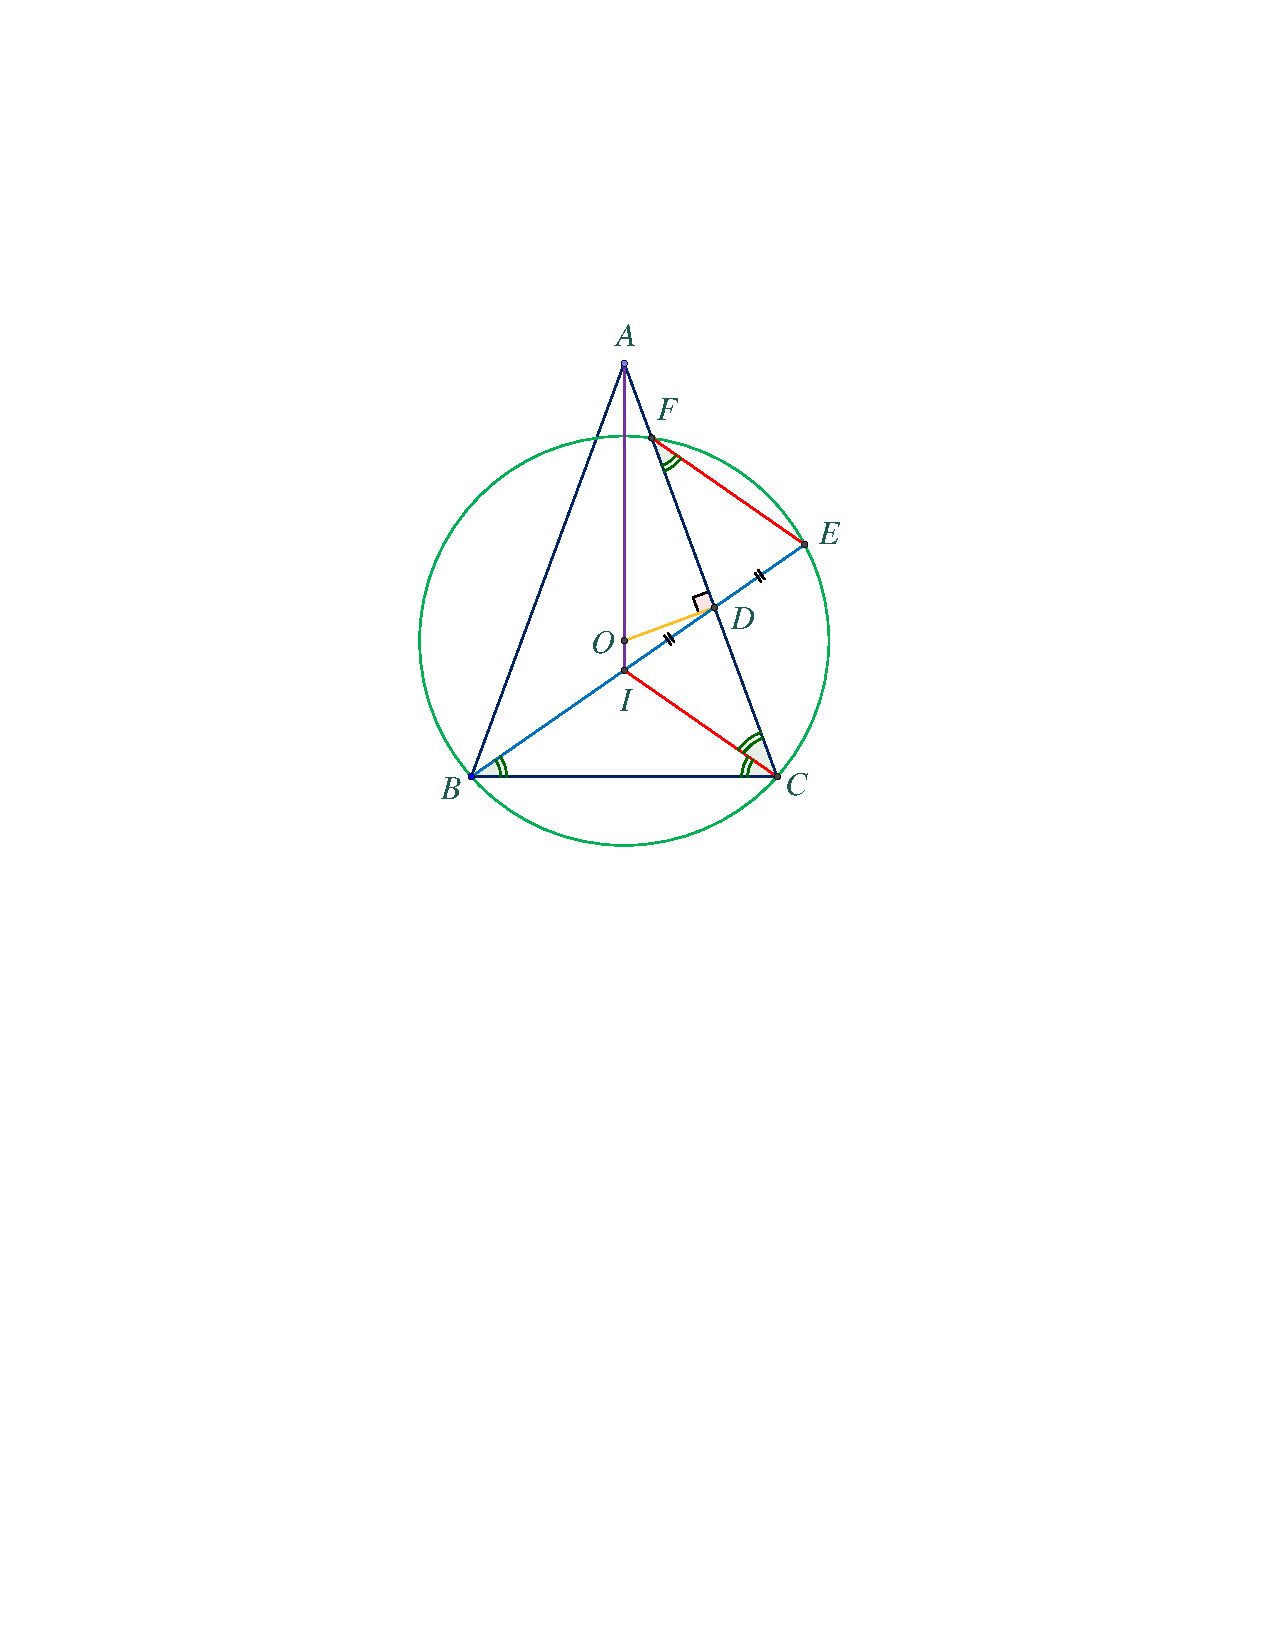
\includegraphics[width= 0.85\linewidth]{P584}
		\vspace*{-15pt}
	\end{figure}
	Gọi $F$ là giao điểm thứ hai của $AC$ và đường tròn $(BCE)$.
	\vskip 0.05cm
	Do $BCEF$ là tứ giác nội tiếp, nên \linebreak $\angle EFC = \angle EBC$. \hfill ($1$)
	\vskip 0.05cm
	Do $I$ là tâm đường tròn nội tiếp tam giác $ABC$ cân tại $A$, nên $BIC$ là tam giác cân tại $I$, và $CI$ là phân giác trong của $\angle BCA$.  Do đó
	\begin{align*}
		&\angle EBC = \angle IBC = \angle ICB. \tag{$2$}\\
		&\angle ICB = \angle ICA = \angle ICF. \tag{$3$}
	\end{align*}
	Từ ($1$), ($2$) và ($3$), suy ra $\angle EFC = \angle ICF$. Do đó, $IC \parallel FE$. Suy ra
	\begin{align*}
		\angle DIC = \angle DEF. \tag{$4$}
	\end{align*}
	Vì $I$ và $E$ đối xứng với nhau qua $D$, nên \linebreak$DI=DE$. \hfill ($5$)
	\vskip 0.05cm
	Lại có 
	\begin{align*}
		\angle IDC = \angle EDF \text{\, \color{black}(hai góc đối đỉnh)}. \tag{$6$}
	\end{align*}
	Từ ($4$), ($5$) và ($6$), suy ra $\Delta IDC=\Delta EDF$  (g.c.g.). Vì thế $DC=DF$, hay $D$ là trung điểm của $CF$. Từ đây, do $O$ là tâm đường tròn đi qua $C, F$, và  $O \not\equiv D$ suy ra $OD\bot CF$, hay $OD\bot AC$.
	\vskip 0.05cm
	Ta có điều phải chứng minh theo yêu cầu đề bài.
	\vskip 0.05cm
	\textbf{\color{thachthuctoanhoc}Bình luận và Nhận xét}
	\vskip 0.05cm
	Tất cả các lời giải Tạp chí nhận được từ bạn đọc đều là lời giải đúng.
	\begin{flushright}
		\textbf{\color{thachthuctoanhoc}Hạ Vũ Anh}
	\end{flushright}
	{\color{thachthuctoanhoc}{\usefont{T5}{qag}{b}{n} P584.}}
	(Mức $B$) Tìm tất cả các số tự nhiên $x, y, z$ thỏa mãn
	\begin{align*}
		(y-z)^4 + 1 = 2^x \cdot yz.
	\end{align*}
	\textbf{\color{thachthuctoanhoc}Lời giải} (\textit{dựa theo cách giải của một bạn học sinh cấp THCS})\textbf{\color{thachthuctoanhoc}.}
	\vskip 0.05cm
	$\bullet$ Giả sử $x, y, z$ là các số tự nhiên thỏa mãn yêu cầu đề bài; nghĩa là, ta có:
	\begin{align*}
		(y-z)^4 + 1 = 2^x \cdot yz. \tag{$1$}
	\end{align*}
	Nhận thấy, nếu $x\ge 1$ thì vế phải của ($1$) là một số chẵn; suy ra $y - z$ là một số lẻ. Do đó $y$ và $z$ khác tính chẵn lẻ. Vì thế $yz$ là một số chẵn; suy ra vế phải của ($1$) là một số chia hết cho $4$. Do đó
	\begin{align*}
		(y-z)^4 + 1 \,\,\vdots\,\, 4. \tag{$2$}
	\end{align*}        
	Vì $y - z$ là số lẻ nên
	\begin{align*}
		{\left( {y - z} \right)^4} - 1 = &\left( {\left( {y - z} \right) - 1} \right)\left( {\left( {y - z} \right) + 1} \right)\\
		&\times\left( {{{\left( {y - z} \right)}^2}\, + 1} \right) \vdots\,\,  4. \tag{$3$}
	\end{align*}
	Từ ($2$) và ($3$) suy ra
	\begin{align*}
		2 = \left( {{{\left( {y - z} \right)}^4} + 1} \right) - \left( {{{\left( {y - z} \right)}^4} - 1} \right) \vdots\,\, 4,
	\end{align*}
	là điều vô lý. Vì vậy $x \not\ge 1$. Do đó $x= 0$.
	\vskip 0.05cm
	Vì $x= 0$ nên từ ($1$) ta được:
	\begin{align*}
		(y-z)^4 + 1 = yz. \tag{$4$}
	\end{align*}
	Đặt $a=y - z$; khi đó ($4$) được viết lại dưới dạng:
	\begin{align*}
		a^4 + 1 = yz. \tag{$5$}
	\end{align*}
	Ta có:
	\begin{align*}
		(5) &\Leftrightarrow 4a^4 + 4 = 4yz \\
		&\Leftrightarrow 4a^4 + 4 = (y+z)^2 - a^2\\
		&\Leftrightarrow 4a^4 + a^2 + 4 = (y+ z)^2.
	\end{align*}
	Do đó $4a^4 + a^2 + 4$  là một số chính \linebreak phương.       \hfill ($6$)
	\vskip 0.05cm
	Hơn nữa, ta có:
	\begin{align*}
		{\left({2{a^2}} \right)^2}\! <\! 4{a^4}\! +\! {a^2}\! + \!4 \!\le\! {\left( {2{a^2}\! +\! 2} \right)^2}.\tag{$7$}
	\end{align*}
	Từ ($6$) và ($7$) suy ra
	\begin{align*}
		\left[ \begin{array}{l}
			4{a^4}\, + {a^2}\, + 4 = {\left( {2{a^2}\, + 1} \right)^2}, \hspace*{48pt} \text{\color{black}(}8\text{\color{black})}\\
			4{a^4}\, + {a^2}\, + 4 = {\left( {2{a^2}\, + 2} \right)^2}.\hspace*{45pt} \text{\color{black}(}9\text{\color{black})}
		\end{array} \right.
	\end{align*}
	Ta có:
	\begin{align*}
		&(8) \!\Leftrightarrow\! 4{a^4}\! +\! {a^2}\! +\! 4 \!=\! 4{a^4}\! +\! 4{a^2}\! + \!1 \!\Leftrightarrow\! a \!=\! \pm\! 1.\\
		&(9) \!\Leftrightarrow\! 4{a^4}\! +\! {a^2}\! +\! 4 \!= \!4{a^4}\! +\! 8{a^2}\! +\! 4 \!\Leftrightarrow \!a \!=\! 0.
	\end{align*}
	Với $a = \pm 1$,  từ ($5$) ta có $yz= 2$; vì thế, với $a= 1$, ta có
	\begin{align*}
		\begin{cases}
			y-z = 1,\\[-0.5ex]
			yz = 2, \tag{$10$}
		\end{cases}
	\end{align*}
	và với $a = -1$  ta có
	\begin{align*}
		\begin{cases}
			y-z = -1,\\[-0.5ex]
			yz = 2. \tag{$11$}
		\end{cases}
	\end{align*}
	Với  $a = 0$, từ ($5$) ta có $yz=1$; vì thế, với $a= 0$, ta có
	\begin{align*}
		\begin{cases}
			y-z = 0\\[-0.5ex]
			yz = 1. \tag{$12$}
		\end{cases}
	\end{align*}
	Từ ($10$) ta được $y= 2$, $z= 1$; từ ($11$) ta được $y= 1$, $z= 2$; và từ ($12$) ta được $y=z=1$.
	\vskip 0.05cm
	Như vậy, nếu $x, y, z$ là các số tự nhiên thỏa mãn yêu cầu đề bài thì: $x\!=\! 0, y\!=\! 2, z\!=\! 1$; $x= 0, y= 1, z= 2; x= 0, y= 1, z= 1$.
	\vskip 0.05cm
	$\bullet$ Ngược lại, bằng phép thử trực tiếp, dễ thấy các bộ ba số vừa nêu trên thỏa mãn các yêu cầu đề bài. Vì vậy, chúng là tất cả các bộ số tự nhiên cần tìm.
	\vskip 0.05cm
	\textbf{\color{thachthuctoanhoc}Bình luận và Nhận xét}
	\vskip 0.05cm
	Trong số các lời giải Tạp chí nhận được từ bạn đọc chỉ có $4$ lời giải đúng và hoàn chỉnh.
	\begin{flushright}
		\textbf{\color{thachthuctoanhoc}Lưu Thị Thanh Hà}
	\end{flushright}
	{\color{thachthuctoanhoc}{\usefont{T5}{qag}{b}{n} P586.}}
	(Mức $B$) Cho $a, b, c$ là các số thực dương có tổng bằng $3$. Chứng minh rằng
	\begin{align*}
		2\left( {\frac{1}{a} + \frac{1}{b} + \frac{1}{c}} \right) \ge {a^2}\, + {b^2}\, + {c^2}\, + 3.
	\end{align*}
	\textbf{\color{thachthuctoanhoc}Lời giải} (\textit{của người chấm bài})\textbf{\color{thachthuctoanhoc}.}
	\vskip 0.05cm
	Do $a+b+c= 3$ nên
	\begin{align*}
		{a^2}\! +\! {b^2}\! +\! {c^2} &= {\left( {a \!+\! b \!+\! c} \right)^2}\! -\! 2\left( {ab \!+\! bc \!+\! ca} \right) \\[-0.5ex]
		&= 9 - 2\left( {ab + bc + ca} \right).
	\end{align*}
	Vì thế bất đẳng thức cần chứng minh theo yêu cầu đề bài được viết lại thành:
	\begin{align*}
		\frac{1}{a} + \frac{1}{b} + \frac{1}{c} \ge 6 - \left( {ab + bc + ca} \right),
	\end{align*}
	hay
	\begin{align*}
		\frac{1}{a} + \frac{1}{b} + \frac{1}{c} + \left( {ab + bc + ca} \right) \ge 6. \tag{$1$}
	\end{align*}
	Tiếp theo, ta sẽ chứng minh ($1$).
	\vskip 0.05cm
	Do $a, b, c$ có vai trò như nhau trong bài toán, nên không mất tổng quát giả sử $a\!\ge\! b\!\ge\! c \!>\!  0$.
	Khi đó ta có
	\begin{align*}
		0 < c \le \frac{{a + b + c}}{3} = 1.
	\end{align*}
	Vì thế
	\begin{align*}
		\frac{1}{c} \!+\! bc \!+\! ca &= \frac{1}{c} + c\left( {a + b} \right) = \frac{1}{c} + c\left( {3 - c} \right) \\[-0.5ex]
		&= \frac{{1 \!+\! 3{c^2}\! -\! {c^3}}}{c} \\
		&= \frac{{{{\left( {1 \!-\! c} \right)}^3}}}{c} \!+\! 3 \!\ge\! 3. \tag{$2$}
	\end{align*}
	Do $a, b >  0$ nên theo bất đẳng thức Cauchy ta có:
	\begin{align*}
		\frac{1}{a} + \frac{1}{b} + ab \ge 3\sqrt[3]{{\frac{1}{a} \cdot \frac{1}{b} \cdot ab}} = 3. \tag{$3$}
	\end{align*}
	Cộng ($2$) và ($3$) theo vế ta thu được ($1$).
	\vskip 0.05cm
	Bất đẳng thức ($1$) được chứng minh; do đó bất đẳng thức của đề bài được chứng minh.
	\vskip 0.05cm
	\textbf{\color{thachthuctoanhoc}Bình luận và Nhận xét}
	\vskip 0.05cm
	$\pmb{1.}$ Qua lời giải trên dễ thấy, dấu đẳng thức ở bất đẳng thức của đề bài xảy ra khi và chỉ khi $a=b=c= 1$.
	\vskip 0.05cm
	$\pmb{2.}$ Bài đã ra cũng chính là một bài toán trong Đề thi của Kỳ thi Junior Balkan Mathematical Olympiad (JBMO) năm $2015$. Phát biểu gốc của bài toán đó là:
	\vskip 0.05cm
	``\textit{Với $a, b, c$ là các số thực dương thay đổi, thỏa mãn $a+b+c= 3$, tìm giá trị nhỏ nhất của biểu thức}
	\begin{align*}
		P = \frac{{2 - {a^3}}}{a} + \frac{{2 - {b^3}}}{b} + \frac{{2 - {c^3}}}{c}.\text{\color{black}"}
	\end{align*}
	$\pmb{3.}$ Tạp chí đã nhận được nhiều lời giải từ bạn đọc. Trong số các lời giải đó, có một số lời giải sai đáng tiếc, do người giải bài chưa nắm vững các kiến thức cơ bản về bất đẳng thức.
	\begin{flushright}
		\textbf{\color{thachthuctoanhoc}Võ Quốc Bá Cẩn}
	\end{flushright}
	{\color{thachthuctoanhoc}{\usefont{T5}{qag}{b}{n} P587.}}
	(Mức $A$) Cho $a, b, c, d, e, f$ là sáu số hạng liên tiếp trong dãy Fibonacci. Trong mặt phẳng tọa độ, lấy các điểm $A(a, b)$, $B(c, d)$, $C(e, f)$. Tính diện tích của tam giác $ABC$.
	\vskip 0.05cm
	(Dãy Fibonacci $(F_n)$  được xác định như sau: $F_0 = 0, F_1 = 1$  và $F_{n+2} = F_{n+1} + F_n$  với mọi $n\ge 0$.)
	\vskip 0.05cm
	\textbf{\color{thachthuctoanhoc}Lời giải} (\textit{dựa theo cách giải của bạn Nguyễn Gia Khánh, lớp $10$ Toán $1$, trường THPT chuyên Hưng Yên, tỉnh Hưng Yên})\textbf{\color{thachthuctoanhoc}.}
	\vskip 0.05cm
	Ký hiệu $S_{ABC}$ là diện tích tam giác $ABC$, ta có:
	\begin{align*}
			&{S_{ABC}} = \frac{1}{2}AB \cdot AC \cdot \sin \angle BAC\\[-0.5ex]
			 = &\frac{1}{2}\left| {\overrightarrow {AB} } \right| \cdot \left| {\overrightarrow {AC} } \right| \cdot \sqrt {1 - {{\cos }^2}\left( {\overrightarrow {AB} ,\overrightarrow {AC} } \right)} \\[-0.5ex]
			 = &\frac{1}{2}\left| {\overrightarrow {AB} } \right| \cdot \left| {\overrightarrow {AC} } \right| \cdot \sqrt {1 - \frac{{{{\left( {\overrightarrow {AB}  \cdot \overrightarrow {AC} } \right)}^2}}}{{{{\left( {\left| {\overrightarrow {AB} } \right| \cdot \left| {\overrightarrow {AC} } \right|} \right)}^2}}}} \\[-0.5ex]
			 = &\frac{1}{2}\sqrt {{{\left( {\left| {\overrightarrow {AB} } \right| \cdot \left| {\overrightarrow {AC} } \right|} \right)}^2}\, - {{\left( {\overrightarrow {AB}  \cdot \overrightarrow {AC} } \right)}^2}}. \tag{$1$}
	\end{align*}
	Do $a, b, c, d, e, f$ là sáu số hạng liên tiếp trong dãy Fibonacci, nên
	\begin{align*}
		&c = a + b, d = a + 2b,\\[-0.4ex]
		&e = 2a + 3b, \text{\color{black}và } f = 3a + 5b.
	\end{align*}
	Do đó
	\begin{align*}
		&\overrightarrow {AB}  = \left( {c - a,d - b} \right) = \left( {b,a + b} \right)\\[-0.4ex]
		\text{\color{black}và}\,\,\, &\overrightarrow {AC}  = \left( {e - a,f - b} \right) = \left( {a + 3b,3a + 4b} \right).
	\end{align*}
	Suy ra
	\begin{align*}
		&\left| {\overrightarrow {AB} } \right| = \sqrt {{b^2}\, + {{\left( {a + b} \right)}^2}},\\[-0.4ex]
		&\left| {\overrightarrow {AC} } \right| = \sqrt {{{\left( {a + 3b} \right)}^2}\, + {{\left( {3a + 4b} \right)}^2}} ,
	\end{align*}
	và
	\begin{align*}
		\overrightarrow {AB}  \cdot \overrightarrow {AC}  = b\left( {a + 3b} \right) + \left( {a + b} \right)\left( {3a + 4b} \right).
	\end{align*}                                      
	Vì thế
	\begin{align*}
		&{\left( {\left| {\overrightarrow {AB} } \right| \cdot \left| {\overrightarrow {AC} } \right|} \right)^2} - {\left( {\overrightarrow {AB}  \cdot \overrightarrow {AC} } \right)^2}\\
		 = \,&{\left( {b\left( {3a + 4b} \right) - \left( {a + b} \right)\left( {a + 3b} \right)} \right)^2}. \tag{$2$}
	\end{align*}
	Từ ($1$) và ($2$) ta được:
	\begin{align*}
		{S_{ABC}} &= \frac{1}{2} \cdot \left| {b\left( {3a + 4b} \right) - \left( {a + b} \right)\left( {a + 3b} \right)} \right| \\
		&= \frac{1}{2} \cdot \left| {{b^2} - ab - {a^2}} \right|. \tag{$3$}
	\end{align*}
	Tiếp theo, với mọi $k \in \mathbb{N^*}$  ta có:
	\begin{align*}
		&\left| {F_{k + 1}^2\, - {F_{k + 1}} \cdot {F_k}\, - F_k^2} \right| \\
		= &\left| {{{\left( {{F_{k - 1}}\, + {F_k}} \right)}^2}\, - \left( {{F_{k - 1}}\, + {F_k}} \right) \cdot {F_k}\, - F_k^2} \right| \\
		= &\left| {F_k^2\, - {F_k} \cdot {F_{k - 1}}\, - F_{k - 1}^2} \right|.
	\end{align*}
	Suy ra
	\begin{align*}
		&\left| {F_k^2\, - {F_k} \cdot {F_{k - 1}}\, - F_{k - 1}^2} \right| \\
		= &\left| {F_1^2\, - {F_1} \cdot {F_0}\, - F_0^2} \right| \\
		= &\left| {{1^2}\, - 1 \cdot 0 - {0^2}} \right| = 1, \tag{$4$}
	\end{align*}
	với mọi $k \in \mathbb{N^*}$
	\vskip 0.05cm 
	Do $a, b$ là hai số hạng liên tiếp trong dãy Fibonacci, nên từ ($3$) và ($4$), ta được:
	\begin{align*}
		{S_{ABC}}\, = \frac{1}{2} \cdot 1 = \frac{1}{2}.
	\end{align*}
	\textbf{\color{thachthuctoanhoc}Bình luận và Nhận xét}
	\vskip 0.05cm
	$\pmb{1.}$ Bài đã ra là một bài toán cơ bản liên quan đến tính chất của dãy Fibonacci, được khéo léo ẩn sau công thức tính diện tích tam giác.
	\vskip 0.05cm
	$\pmb{2.}$ Rất tiếc, trong số các lời giải Tạp chí đã nhận được từ bạn đọc, có năm lời giải sai, do người giải bài đã mắc một trong các sai sót sau:
	\vskip 0.05cm
	$\bullet$ \textit{Sai kiến thức cơ bản}. Chẳng hạn, có hai bạn học sinh lớp 8 THCS đã viết:
	\begin{align*}
		{S_{ABC}}\, = \frac{1}{2}\left| {\left[ {\overrightarrow {AB} ,\overrightarrow {AC} } \right]} \right|.
	\end{align*}
	(\textit{\textbf{\color{thachthuctoanhoc}Lưu ý} rằng, \textbf{\color{thachthuctoanhoc}không} có khái niệm tích có hướng đối với các vectơ trong mặt phẳng. Ở bài toán đã ra, các điểm $A$, $B$ được cho trong mặt phẳng tọa độ; vì thế, không có tích có hướng}  $\left[ {\overrightarrow {AB} ,\overrightarrow {AC} } \right]$.)
	\vskip 0.05cm
	$\bullet$ \textit{Thực hiện sai các biến đổi}. Chẳng hạn, có bạn đã biến đổi như sau: “$b - (3a + 5b) = -2a - 5b$”.
	\vskip 0.05cm
	$\bullet$ Kết thúc lời giải khi \textit{chưa tính được diện tích tam giác} $ABC$. Chẳng hạn, có bạn đã kết thúc lời giải khi mới chỉ chứng minh được ${S_{ABC}}\, = \frac{1}{2} \cdot \left| {{b^2}\, - ab - {a^2}} \right|$.
	\vskip 0.05cm
	$\pmb{3.}$ Nhân sai sót về kiến thức cơ bản nêu trên, người chấm bài này cho rằng, \textbf{\textit{\color{thachthuctoanhoc}rất nên tránh}} việc trang bị quá sớm cho học sinh các kiến thức của lớp trên. Vì việc trang bị như thế có thể vừa tạo ra những lỗ hổng trong kiến thức, vừa làm mất đi quá trình kiến tạo kiến thức của học sinh.
	\vskip 0.05cm
		\hfill \textbf{\color{thachthuctoanhoc}Trần Nam Dũng}
	\vskip 0.05cm
	{\color{thachthuctoanhoc}{\usefont{T5}{qag}{b}{n} P588.}}
	(Mức $A$) Xét các số thực $x, y, z$ thỏa mãn
	\begin{align*}
		{\left( {x - 1} \right)^2}\, + {\left( {y + 2} \right)^2}\, + {\left( {z - 1} \right)^2}\, = 300.
	\end{align*}
	Tìm giá trị lớn nhất và giá trị nhỏ nhất của biểu thức
	\begin{align*}
		P = \left[ {{x^2}} \right] + \left[ {{y^2}} \right] + \left[ {{z^2}} \right].
	\end{align*}
	\textbf{\color{thachthuctoanhoc}Lời giải} (\textit{dựa theo cách giải của bạn Nguyễn Hùng Cường, $297$ Nguyễn Thị Minh Khai, Tp. Qui Nhơn, Tỉnh Bình Định})\textbf{\color{thachthuctoanhoc}.}
	\vskip 0.05cm
	Đặt $a=x - 1, b=y+ 2$ và $c=z - 1$; theo giả thiết, ta có:
	\begin{align*}
		a^2 + b^2 + c^2 = 300, \tag{$1$}
	\end{align*}
	và
	\begin{align*}
		P = \left[ {{{\left( {a + 1} \right)}^2}} \right] + \left[ {{{\left( {b - 2} \right)}^2}} \right] + \left[ {{{\left( {c + 1} \right)}^2}} \right].
	\end{align*}
	Vì với mọi số thực $x$, $x - 1 < [x]  \le x$, nên
	\begin{align*}
		&{\left( {a + 1} \right)^2} + {\left( {b - 2} \right)^2} + {\left( {c + 1} \right)^2}\, - 3 < P \\
		\le \,&{\left( {a + 1} \right)^2} + {\left( {b - 2} \right)^2} + {\left( {c + 1} \right)^2}. \tag{$2$}
	\end{align*}
	Vì
	\begin{align*}
		&{\left( {a + 1} \right)^2} + {\left( {b - 2} \right)^2} + {\left( {c + 1} \right)^2}\\
		 = \,&\left( {{a^2} + {b^2} + {c^2}} \right) + 2\left( {a - 2b + c} \right) + 6,
	\end{align*}
	nên từ ($1$) và ($2$), ta được:
	\begin{align*}
		&303 + 2\left( {a - 2b + c} \right) < P \\
		\le \,&306 + 2\left( {a - 2b + c} \right). \tag{$3$}
	\end{align*}
	Áp dụng bất đẳng thức Bunhiacopski cho hai bộ ba số thực $(a, b, c)$, $(1, -2, 1)$, và sử dụng ($1$), ta có:
	\begin{align*}
		{\left( {a \!-\! 2b \!+\! c} \right)^2}\!\le \!&\left(\!{{1^2}\! +\! {{\left( { \!-\! 2} \right)}^2} \!+\! {1^2}} \!\right)\!\!\left(\!{{a^2} \!+\! {b^2} \!+\! {c^2}} \!\right)\\
		= &6 \cdot 300 = 1800.
	\end{align*}
	Do đó
	\begin{align*}
		 - 30\sqrt 2  \le a - 2b + c \le 30\sqrt 2 . \tag{$4$}
	\end{align*}
	Từ ($3$) và ($4$), suy ra
	\begin{align*}
		303 - 60\sqrt 2  < P \le 306 + 60\sqrt 2 . \tag{$5$}
	\end{align*}
	Vì  $\sqrt{2} < \frac{17}{12}$ nên từ ($5$) suy ra $218 <P< 391$. Từ đây, do $P$ là số nguyên, ta có:
	\begin{align*}
		219 \le P \le 390.
	\end{align*}
	Hơn nữa, với  $x=z = -5{,}8$, $y =- 2 + \sqrt{207{,}52}$  ta có
	\begin{align*}
		&{\left( {x - 1} \right)^2} + {\left( {y + 2} \right)^2} + {\left( {z - 1} \right)^2}\\
		= \,&{\left( { \!-\! 6,8} \right)^2} \!+\! {\left( \!{\sqrt {207,52} } \right)^2} \!+\! {\left( { \!-\! 6,8} \right)^2} \!=\! 300,
	\end{align*}
	\begin{align*}
		P =& \left[ {{{\left( { - 5,8} \right)}^2}} \right] + \left[ {{{\left( { - 2 + \sqrt {207,52} } \right)}^2}} \right] \\[-0.3ex]
		&+ \left[ {{{\left( {{{\left( { - 5,8} \right)}^2}} \right)}^2}} \right]\\[-0.3ex]
		=& \left[ {33,64} \right] + \left[ {211,52 - 4\sqrt {207,52} } \right] \\[-0.3ex]
		&+ \left[ {33,64} \right]\\[-0.3ex]
		=& 33 + 153 + 33 = 219;
	\end{align*}
	và với  $x=z = 8$, $y = -2-\sqrt{202}$,  ta có
	\begin{align*}
		&{\left( {x - 1} \right)^2}\, + {\left( {y + 2} \right)^2}\, + {\left( {z - 1} \right)^2}\\
		 = \,&\,{7^2} + {\left( {\sqrt {202} } \right)^2} + {7^2} = 300,\\
		= \,&\left[ {{8^2}} \right] + \left[ {{{\left( { - 2 - \sqrt {202} } \right)}^2}} \right] + \left[ {{8^2}} \right]\\
		= \,&\,64 + 262 + 64 = 390.
	\end{align*}
	Vì vậy, giá trị nhỏ nhất và giá trị lớn nhất của $P$, tương ứng, bằng $219$ và $390$.
	\vskip 0.05cm
	\textbf{\color{thachthuctoanhoc}Bình luận và Nhận xét}
	\vskip 0.05cm
	Lời giải của bạn \textit{Nguyễn Hùng Cường} là lời giải duy nhất Tạp chí nhận được từ bạn đọc.
	\begin{flushright}
		\textbf{\color{thachthuctoanhoc}Lê Huy}
	\end{flushright}
	{\color{thachthuctoanhoc}{\usefont{T5}{qag}{b}{n} P589.}}
	(Mức $A$) Cho tam giác nhọn $ABC$ nội tiếp đường tròn $(O)$, có trực tâm $H$, và $M$ là trung điểm $BC$. Qua $H$, kẻ đường thẳng $d$, lần lượt cắt các cạnh $AB$, $AC$ tại $F$, $E$. Gọi $K$ là tâm đường tròn ngoại tiếp tam giác $AEF$, và $J$ là trung điểm $EF$. Các đường thẳng $AK$, $AJ$ tương ứng cắt $(O)$ tại các điểm thứ hai $L$, $G$. Chứng minh rằng $\angle MLG = 90^\circ$.
	\vskip 0.05cm 
	\textbf{\color{thachthuctoanhoc}Lời giải} (\textit{dựa theo cách giải của bạn Hồ Trần Khánh Linh, lớp $11$ Toán $2$, trường THPT chuyên Sư phạm, ĐH Sư phạm Hà Nội})\textbf{\color{thachthuctoanhoc}.}
	\vskip 0.05cm
	Trước hết, ta nhắc lại (không chứng minh) kết quả cơ bản sau:
	\vskip 0.05cm
	\textbf{\color{thachthuctoanhoc}Bổ đề.} Cho hai đường tròn $(O_1), (O_2)$ cắt nhau tại hai điểm phân biệt $A, B$. Một đường thẳng, đi qua $B$, cắt lại $(O_1), (O_2)$, tương ứng, tại $M, N$ ($M \ne A, B; N \ne A, B$). Khi đó, tam giác $AMN$ và tam giác $AO_1O_2$  đồng dạng cùng hướng.
	\vskip 0.05cm
	\textit{Trở lại bài toán.}
	\vskip 0.05cm
	Ký hiệu ($K$) là đường tròn ngoại tiếp tam giác $AEF$.
	\vskip 0.05cm
	Xét hai trường hợp sau:
	\vskip 0.05cm
	$\bullet$ \textit{Trường hợp} $1$: $d \parallel BC$. (Xem Hình $1$)
	\vskip 0.05cm	
	Trong trường hợp này, hai đường tròn, $(O)$ và $(K)$, tiếp xúc trong với nhau tại $A$. Do đó, tồn tại phép vị tự $f$ tâm $A$, biến đường tròn $(K)$ thành đường tròn $(O)$. Qua $f$, $F \mapsto B$, $E \mapsto C$  và $K \mapsto O$.
	\begin{figure}[H]
		\vspace*{-5pt}
		\centering
		\captionsetup{labelformat= empty, justification=centering}
		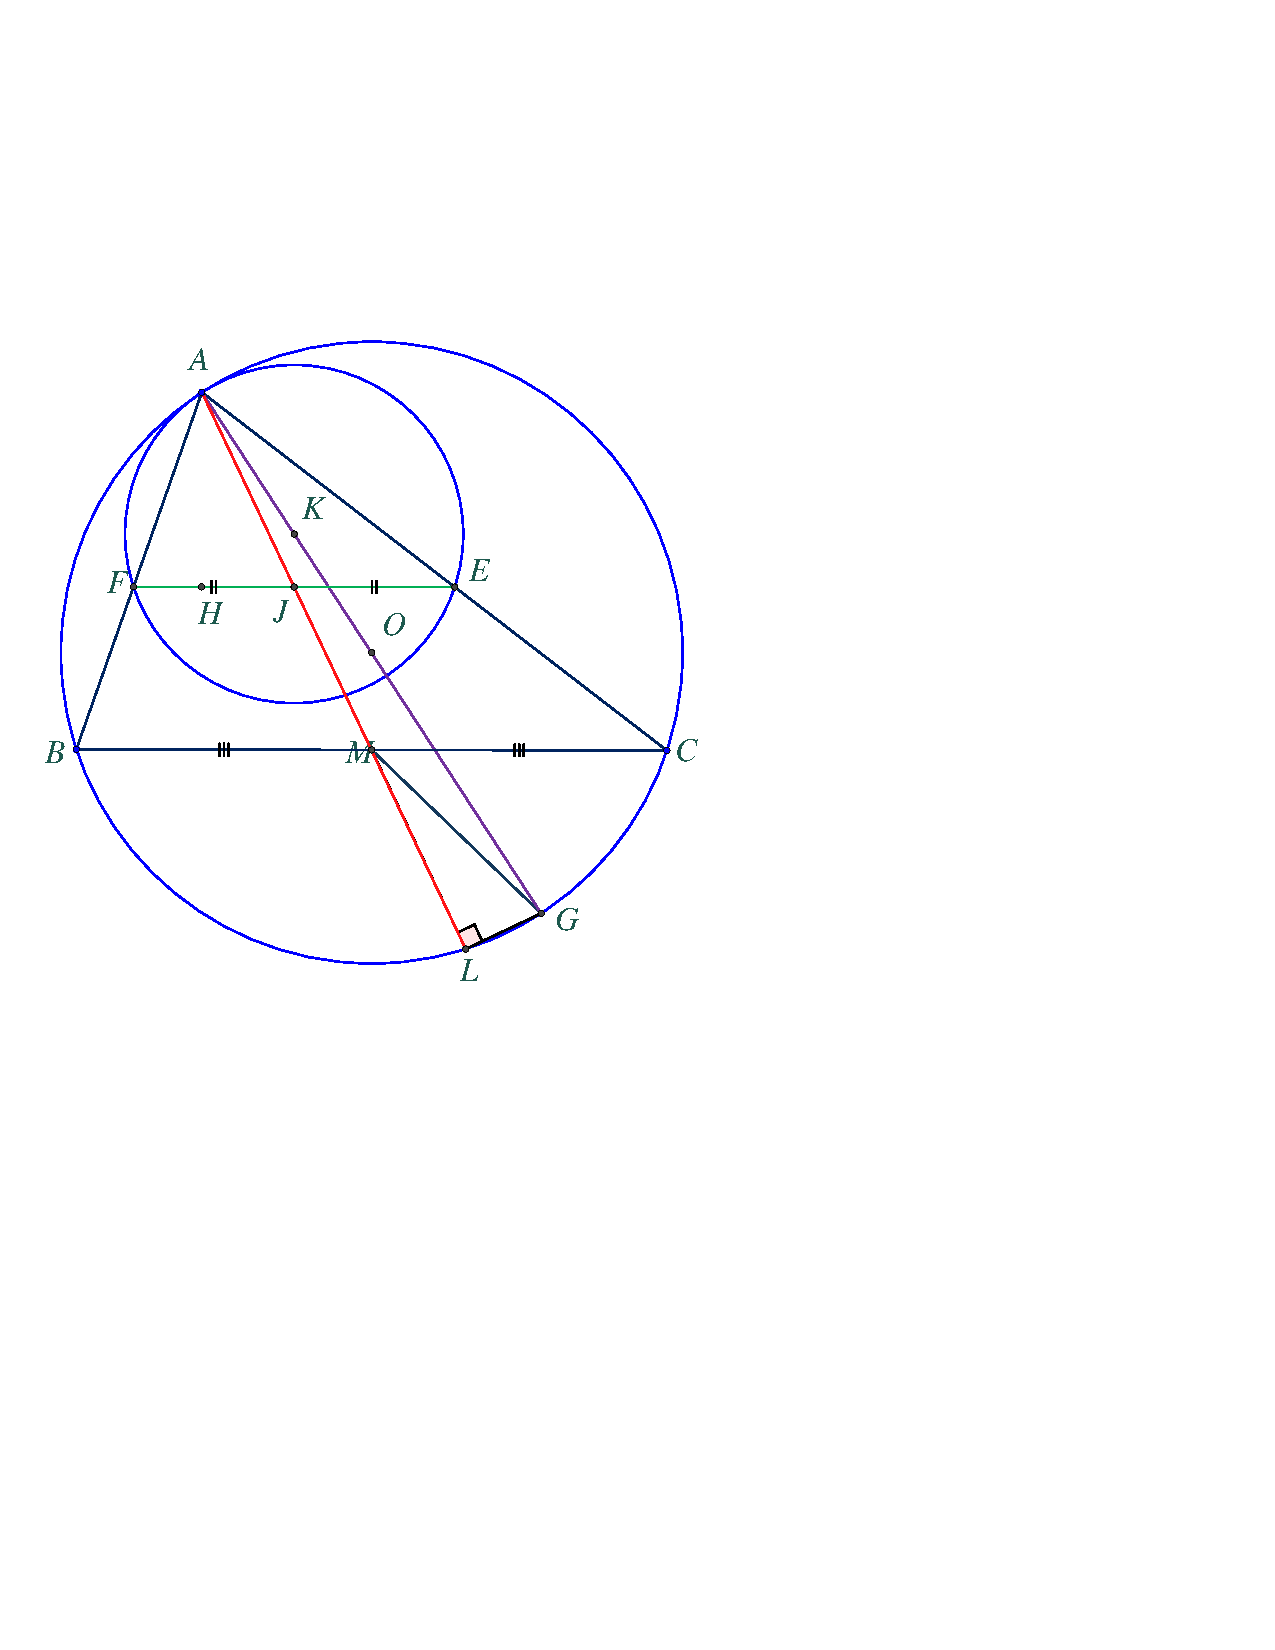
\includegraphics[width= 0.85\linewidth]{P591H1}
		\caption{\small\textit{\color{thachthuctoanhoc}Hình $1$.}}
		\vspace*{-10pt}
	\end{figure}
	Vì $F \mapsto B$, $E \mapsto C$, nên $f$ biến trung điểm $J$ của $FE$ thành trung điểm $M$ của $BC$. Mà $A, J, L$ thẳng hàng, nên $A, M, L$ thẳng hàng. Vì thế, $\angle MLG = \angle ALG$ \hfill ($1$)
	\vskip 0.05cm
	Vì qua $f$, $K \mapsto O$  mà $A, K, G$ thẳng hàng, nên $A, O, G$ thẳng hàng. Do đó, $AG$ là đường kính của $(O)$. Từ đây và ($1$), suy ra 
	\begin{align*}
		\angle MLG = 90^\circ.
	\end{align*}
	$\bullet$ \textit{Trường hợp} $2$: $d$ \textit{không song song với} $BC$. (Xem Hình $2$)
	\begin{figure}[H]
		\vspace*{-5pt}
		\centering
		\captionsetup{labelformat= empty, justification=centering}
		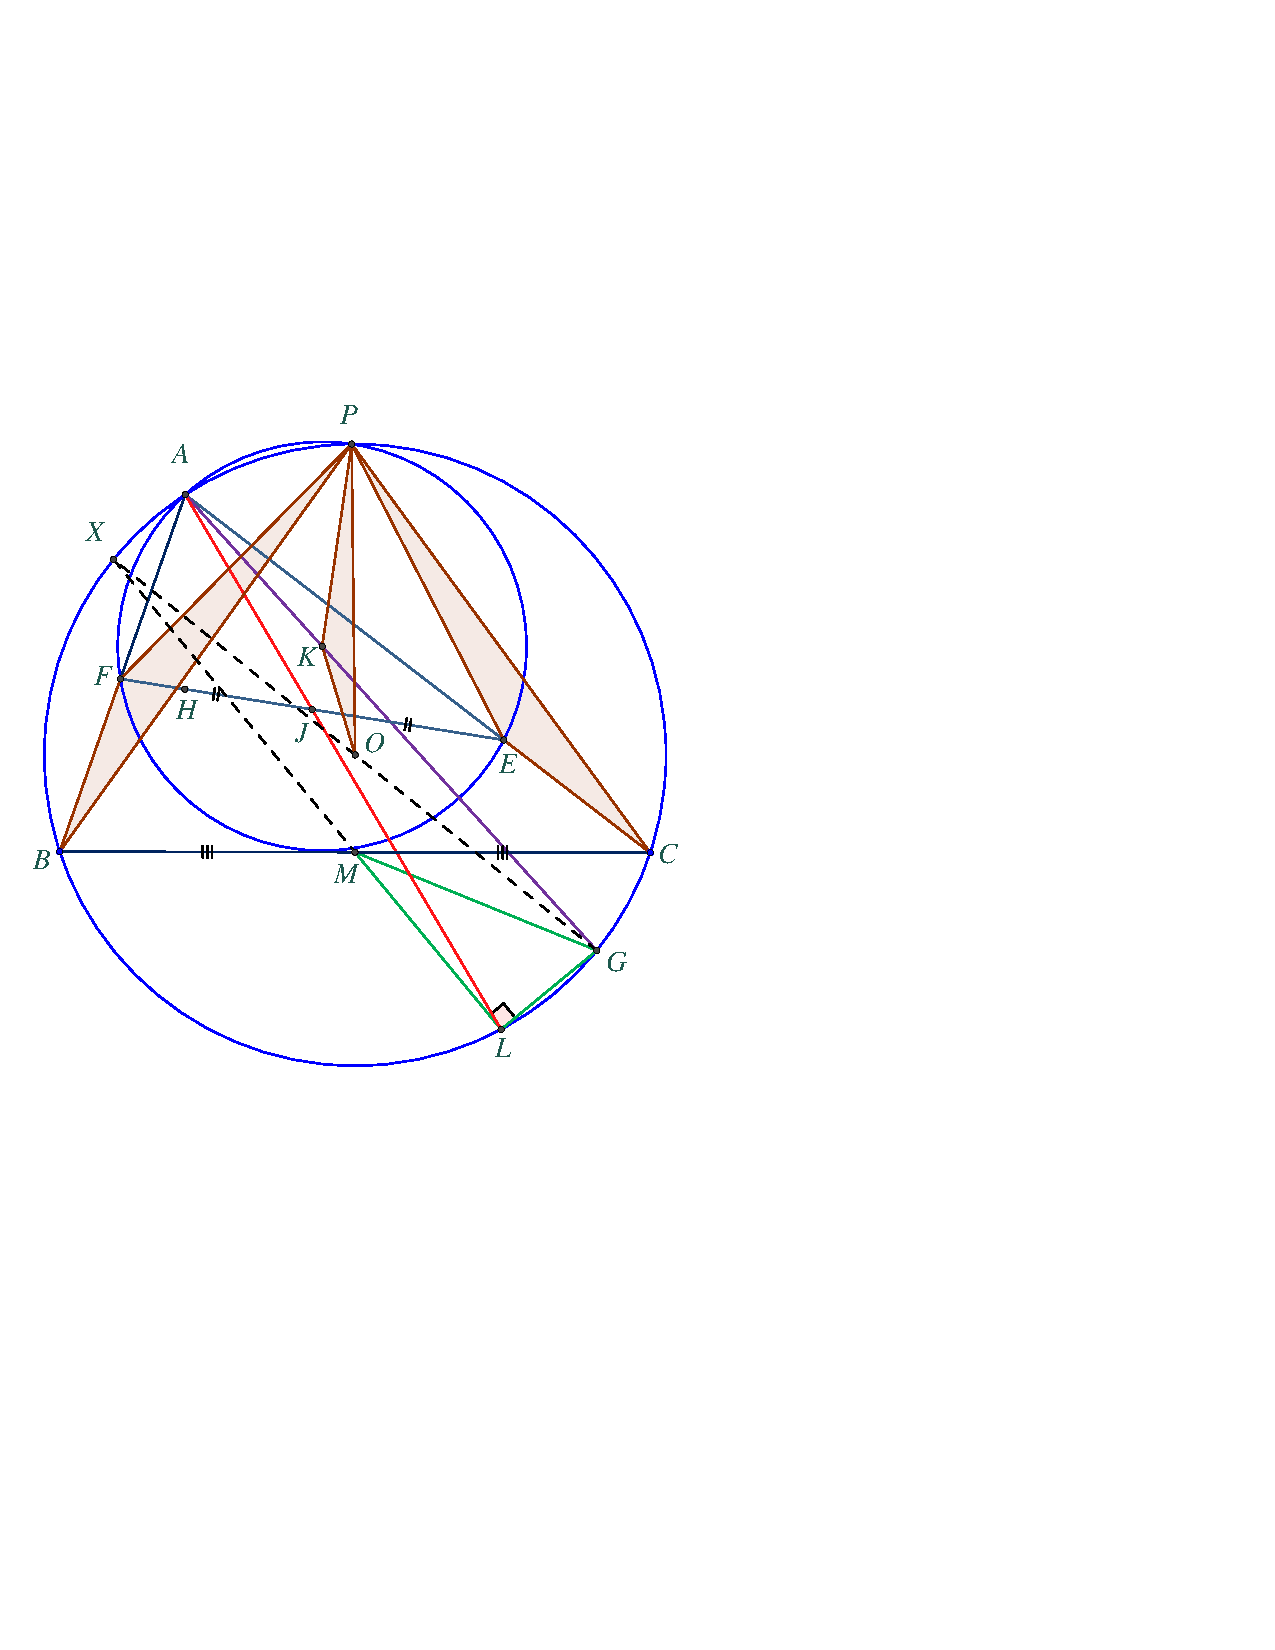
\includegraphics[width= 0.85\linewidth]{P591H2}
		\caption{\small\textit{\color{thachthuctoanhoc}Hình $2$.}}
		\vspace*{-10pt}
	\end{figure}
	Trong trường hợp này, hai đường tròn, $(O)$ và $(K)$, cắt nhau tại hai điểm phân biệt, và một trong hai giao điểm là $A$. Gọi $P$ là giao điểm còn lại.
	\vskip 0.05cm
	Áp dụng Bổ đề cho hai đường tròn $(O)$ và $(K)$, ta được: tam giác $PFB$ và tam giác $PKO$ đồng dạng cùng hướng; tam giác $PEC$ và tam giác $PKO$ đồng dạng cùng hướng. Suy ra, tam giác $PFB$ và tam giác $PEC$ đồng dạng cùng hướng. Do đó, tồn tại phép vị tự quay $g$ tâm $P$, biến tam giác $PFE$ thành tam giác $PBC$. Mà $J, M$ tương ứng là trung điểm của $FE$, $BC$, và $K$, $O$ tương ứng là tâm đường tròn ngoại tiếp tam giác $PFE$, tam giác $PBC$, nên $g$ biến $J$ thành $M$, và $K$ thành $O$. Do đó, tam giác $PJM$ đồng dạng cùng hướng với tam giác $PKO$. Suy ra, tam giác $PJM$ đồng dạng cùng hướng với tam giác $PFB$.
	\vskip 0.05cm
	Vì $\Delta PFB \sim  \Delta PKO$ nên
	\begin{align*}
		\angle POK \!=\! \angle PBF \!=\! \angle PBA \!=\! \angle PGA \!=\! \angle PGK.
	\end{align*}
	Do đó, $PKOG$ là tứ giác nội tiếp; suy ra
	\begin{align*}
		\angle OGK = \angle OPK = \angle BPF. \tag{$2$}
	\end{align*}
	Một cách tương tự, từ $\Delta PFB \sim \Delta PJM$ suy ra, $PJML$ là tứ giác nội tiếp; và do đó,  $\angle MLJ = \angle BPF$.   \hfill ($3$)
	\vskip 0.05cm
	Từ ($2$) và ($3$) ta có $\angle OGK = \angle MLJ$, hay $\angle OGA = \angle MLA$. Suy ra, $GO$ và $LM$ cắt nhau tại một điểm $X$ thuộc $(O)$. Vì thế
	\begin{align*}
		\angle MLG = \angle XLG = 90^\circ
	\end{align*}
	(do $XG$ là đường kính của $(O)$.)
	\vskip 0.05cm
	\textbf{\color{thachthuctoanhoc}Bình luận và Nhận xét}
	\vskip 0.05cm
	$\pmb{1.}$ Bạn \textit{Hồ Trần Khánh Linh} nhận xét đúng rằng, lời giải trên vẫn giữ nguyên tính đúng, khi $d$ là đường thẳng tùy ý, cắt đồng thời hai cạnh $AB$, $AC$ tương ứng tại các điểm $F, E$, với $F \ne A, B$ và $E \ne A, C$. Vì thế, giả thiết $d$ đi qua trực tâm $H$ của tam giác $ABC$ là một giả thiết thừa.
	\vskip 0.05cm
	$\pmb{2.}$ Trong số các lời giải Tạp chí đã nhận được từ bạn đọc, chỉ có ba lời giải đúng; tất cả các lời giải còn lại đều thiếu xét trường hợp $d \parallel BC$.
	\begin{flushright}
		\textbf{\color{thachthuctoanhoc}Hạ Vũ Anh}
	\end{flushright}
	{\color{thachthuctoanhoc}{\usefont{T5}{qag}{b}{n} P590.}}
	(Mức $A$) Cho biết, $\{1; 2; 3; 4; 5; 6; 7;$ \linebreak$8; 9\}$ là tập hợp tất cả các hệ số của ba tam thức bậc hai $f(x), g(x), h(x)$. Hỏi, có thể xảy ra hay không, trường hợp ba tam thức đó có nghiệm hữu tỷ chung?
	\vskip 0.05cm
	\textbf{\color{thachthuctoanhoc}Lời giải} (\textit{dựa theo cách giải của Đáp án do BBT Tạp chí cung cấp})\textbf{\color{thachthuctoanhoc}.}
	\vskip 0.05cm
	Xét tam thức bậc hai với hệ số nguyên dương $\varphi \left( x \right) = a{x^2}\, + bx + c$. Ta có các Nhận xét đơn giản và dễ thấy sau:
	\vskip 0.05cm
	$\bullet$ \textit{Nhận xét} $1$. Nếu tam thức $\varphi \left( x \right)$  có nghiệm thực thì $b \ne 1$, và tất cả các nghiệm của nó đều là số âm.
	\vskip 0.05cm
	$\bullet$ \textit{Nhận xét} $2$. Nếu tam thức $\varphi \left( x \right)$  có nghiệm hữu tỷ $x = \alpha$ thì tam thức ${\varphi ^ * }\left( x \right) = c{x^2}\, + bx + a$  có nghiệm hữu tỷ  $x = 1/\alpha$.
	\vskip 0.05cm
	$\bullet$ \textit{Nhận xét} $3$. Nếu $a = 1$ và tam thức $\varphi \left( x \right)$ có nghiệm hữu tỷ thì tất cả các nghiệm của nó đều là số nguyên.
	\vskip 0.05cm
	$\bullet$ \textit{Nhận xét} $4$. Nếu tam thức $\varphi \left( x \right)$  có nghiệm nguyên lẻ thì tổng $a + b + c$ là một số nguyên dương chẵn.
	\vskip 0.05cm
	\textit{Trở lại bài toán.}
	\vskip 0.05cm
	Giả sử tồn tại ba tam thức bậc hai thỏa mãn điều kiện bài toán, và đồng thời, có nghiệm hữu tỷ chung.
	Khi đó, theo các Nhận xét $1$ và $2$, sẽ tồn tại ba tam thức bậc hai
	\begin{align*}
		&f\left( x \right) = {a_1}{x^2}\, + {b_1}x + {c_1}\\
		&g\left( x \right) = {a_2}{x^2}\, + {b_2}x + {c_2}\\
		&h\left( x \right) = {a_3}{x^2}\, + {b_3}x + {c_3}
	\end{align*}
	thỏa mãn điều kiện bài toán (tức, có tập hợp các hệ số của cả ba tam thức là tập $9$ số nguyên dương đầu tiên), và một trong ba hệ số $a_1, a_2, a_3$  bằng $1$; đồng thời, cả ba tam thức đó có nghiệm hữu tỷ chung. Ký hiệu nghiệm này là $x_0$.
	\vskip 0.05cm 
	Vì vai trò của ba tam thức $f(x), g(x), h(x)$ là như nhau, nên không mất tính tổng quát, có thể giả sử $a_1 =1$. Khi đó, vì $x_0$  là nghiệm hữu tỷ của $f(x)$  nên theo các Nhận xét $1$ và $3$, $x_0$  là một số nguyên âm.
	\vskip 0.05cm
	Nhận thấy, nếu $x_0$  là số nguyên âm lẻ thì theo Nhận xét $4$, với mọi $i \in \{1; 2; 3\}$, tổng $a_i + b_i + c_i$ là một số nguyên dương chẵn. Dẫn tới
	\begin{align*}
		\sum\limits_{i = 1}^3 {\left( {{a_i}\, + {b_i}\, + {c_i}} \right)}  = \sum\limits_{k = 1}^9 k  = 45
	\end{align*}
	là một số nguyên dương chẵn. Điều vô lý này cho thấy, $x_0$ không thể là số nguyên âm lẻ. Do vậy, $x_0$  là một số nguyên âm chẵn. \hfill ($1$)
	\vskip 0.05cm
	Tiếp theo, do $x_0$  là nghiệm nguyên chung của $f(x), g(x), h(x)$  nên  $|x_0|$ là ước dương chung của $c_1 , c_2, c_3$. Từ đây, do $\{c_1;c_2;c_3\}$ là tập con của tập $9$ số nguyên dương đầu tiên, suy ra $|x_0| < 4$, hay $x_0 > -4$ (vì nếu ngược lại, $|x_0| \ge 4$,  thì trong tập $9$ số nguyên dương đầu tiên có ít nhất ba số khác nhau cùng chia hết cho một số nguyên dương lớn hơn hoặc bằng $4$, là điều vô lý).    \hfill ($2$)
	\vskip 0.05cm
	Từ ($1$) và ($2$) suy ra, $x_0 = -2$. Do đó, ta có
	\begin{align*}
		4 - 2{b_1} + {c_1} &= 4{a_2} - 2{b_2} + {c_2} \\
		&= 4{a_3} - 2{b_3} + {c_3} = 0. \tag{$3$}
	\end{align*}
	Suy ra, ${c_1},{c_2},{c_3}\, \in S = \left\{ {2;4;6;8} \right\}$. \hfill ($4$)
	\vskip 0.05cm
	Do trong tập $S$ chỉ có hai số không chia hết cho $4$, nên tồn tại $i \in \{1; 2; 3\}$, sao cho $c_i$ chia hết cho $4$. Khi đó, từ ($3$) suy ra,  $b_i$ phải là số chẵn, tức $b_i \in S$. Từ đây và ($4$) suy ra, $a_2$  và $a_3$ là các số nguyên dương lẻ lớn hơn $1$. Do đó, trong hai số vừa nêu, phải có một số không nhỏ hơn $5$. Không mất tổng quát, giả sử $a_2 \ge 5$.  Khi đó, theo ($3$), ta có:
	\begin{align*}
		0 \!=\! 4{a_2}\! -\! 2{b_2}\! +\! {c_2}\! >\! 20 \!-\! 2{b_2}\! >\! 0 \,\,\,(\text{\color{black}do } b_2 \!\le\! 9)
	\end{align*}
	là điều vô lý.
	\vskip 0.05cm
	Điều vô lý vừa nhận được ở trên cho thấy, \textit{không tồn tại} ba tam thức bậc hai thỏa mãn điều kiện đề bài và đồng thời có nghiệm hữu tỷ chung.
	\vskip 0.05cm
	\textbf{\color{thachthuctoanhoc}Bình luận và Nhận xét}
	\vskip 0.05cm
	$\pmb{1.}$ Bài đã ra là một bài toán hay, thú vị. Qua lời giải trên có thể thấy, bài toán được hình thành từ việc khai thác các tính chất rất đơn giản, cơ bản của tam thức bậc hai với hệ số nguyên dương.
	\vskip 0.05cm
	$\pmb{2.}$ Lời giải của bạn \textit{Nguyễn Gia Khánh} (lớp $10$ Toán $1$, trường THPT chuyên Hưng Yên, tỉnh Hưng Yên) là lời giải duy nhất mà Tạp chí nhận được từ bạn đọc. Lời giải của bạn Khánh là một lời giải đúng và hoàn chỉnh.
	\begin{flushright}
		\textbf{\color{thachthuctoanhoc}Nguyễn Khắc Minh}
	\end{flushright}
\end{multicols}
\begin{center}
	\textbf{\color{thachthuctoanhoc}DANH SÁCH HỌC SINH CÓ LỜI GIẢI HOÀN CHỈNH}
\end{center}
\begin{multicols}{2}
	\textit{Trong các ngoặc đơn ở phần dưới đây, sau tên lớp là mã hiệu của các bài toán mà học sinh có lời giải hoàn chỉnh.}
	\vskip 0.05cm
	\textbf{\color{thachthuctoanhoc}KHỐI THCS}
	\vskip 0.05cm
	$\bullet$ Trường \textbf{\color{thachthuctoanhoc}TH, THCS Victoria Thăng Long}, Huyện Thanh Oai, Tp. Hà Nội: \textit{Phạm Minh Anh} (lớp $8$V$1$; P$586$).
	\vskip 0.05cm
	$\bullet$ Trường \textbf{\color{thachthuctoanhoc}TH, THCS \& THPT Archimedes Đông Anh}, Tp. Hà Nội: \textit{Nguyễn Quốc Anh} (lớp $8$A$1$; P$583$, P$586$), \textit{Trần Việt Anh} (lớp $8$C$1$; P$583$, P$584$, P$586$), \textit{Vũ Bảo Lân} (lớp $7$C$2$; P$583$).
	\vskip 0.05cm
	$\bullet$ Trường \textbf{\color{thachthuctoanhoc}THPT chuyên Hà Nội -- Amsterđam}, Tp. Hà Nội: \textit{Hà Mạnh Hùng} (lớp $7$A; P$585$, P$587$).
	\vskip 0.05cm
	$\bullet$ Trường \textbf{\color{thachthuctoanhoc}THCS Trưng Vương}, Quận Hoàn Kiếm, Tp. Hà Nội: \textit{Nguyễn Hoàng Minh} (lớp $9$C$1$; P$586$).
	\vskip 0.05cm
	$\bullet$ Trường \textbf{\color{thachthuctoanhoc}THCS Nguyễn Trãi}, Huyện Đại Lộc, Tỉnh Quảng Nam: \textit{Nguyễn Châu Tuấn Kiệt} (lớp $9/7$; P$583$, P$584$, P$585$, P$586$).
	\vskip 0.05cm
	\textbf{\color{thachthuctoanhoc}KHỐI THPT}
	\vskip 0.05cm
	$\bullet$ Trường \textbf{\color{thachthuctoanhoc}THPT số $\pmb{2}$ Phù Cát}, Tỉnh Bình Định: \textit{Nguyễn Hữu Trí} (lớp $10$A$1$; P$584$, P$586$).
	\vskip 0.05cm
	$\bullet$ Trường \textbf{\color{thachthuctoanhoc}THPT chuyên Lý Tự Trọng}, Tp. Cần Thơ: \textit{Đặng Hoàng Khang} (lớp $10$A$1$B; P$584$).
	\vskip 0.05cm
	$\bullet$ Trường \textbf{\color{thachthuctoanhoc}THPT chuyên Nguyễn Quang Diêu}, Tỉnh Đồng Tháp: \textit{Nguyễn Chí Việt Khang} (lớp $11$T$1$; P$583$, P$584$, P$585$, P$586$, P$587$, P$589$).
	\vskip 0.05cm
	$\bullet$ Trường \textbf{\color{thachthuctoanhoc}THPT Gia Định}, Tp. Hồ Chí Minh: \textit{Lê Anh Khoa} (lớp $10$CT; P$586$), \textit{Nguyễn Hà Ngọc Uyên} (lớp $11$CT; P$584$).
	\vskip 0.05cm
	$\bullet$ Trường \textbf{\color{thachthuctoanhoc}THPT chuyên Hưng Yên}, Tỉnh Hưng Yên: \textit{Nguyễn Gia Khánh} (lớp $10$ Toán $1$; P$587$, P$590$).
	\vskip 0.05cm
	$\bullet$ Trường \textbf{\color{thachthuctoanhoc}THPT chuyên Lê Hồng Phong}, Tỉnh Nam Định: \textit{Nguyễn Đức Khải} (lớp $10$ Toán $2$; P$583$, P$584$, P$586$), \textit{Ninh Thị Mai Linh} (lớp $11$ Toán $1$; P$584$), \textit{Đồng Đức Mạnh} (lớp $10$ Toán $1$; P$584$, P$587$), \textit{Trần Đình Nam} (lớp $10$ Toán $2$; P$583$, P$586$), \textit{Hà Thị Kim Oanh} (lớp $11$ Toán $2$; P$583$, P$584$).
	\vskip 0.05cm
	$\bullet$ Trường \textbf{\color{thachthuctoanhoc}THPT chuyên Lương Văn Chánh}, Tỉnh Phú Yên: \textit{Nguyễn Thị Bảo Tiên} (lớp $10$ Toán $1$; P$584$, P$586$).
	\vskip 0.05cm
	$\bullet$ Trường \textbf{\color{thachthuctoanhoc}THPT chuyên Quốc học}, Tỉnh Thừa Thiên -- Huế: \textit{Võ Minh Hiển} (lớp $10$ Toán $1$; P$584$), \textit{Đỗ Đại Phong} (lớp $10$ Toán $1$; P$584$), \textit{Trần Thị Thanh Thư} (lớp $11$ Toán $1$; P$582$).
	\vskip 0.05cm
	$\bullet$ Trường \textbf{\color{thachthuctoanhoc}THPT chuyên Khoa học tự nhiên}, ĐH Khoa học tự nhiên -- ĐHQG Hà Nội: \textit{Nguyễn Cung Thành} (lớp $10$A$1$ Toán; P$583$, P$584$, P$586$, P$587$, P$589$).
	\vskip 0.05cm
	$\bullet$ Trường \textbf{\color{thachthuctoanhoc}THPT chuyên Sư phạm}, ĐH Sư phạm Hà Nội: \textit{Hồ Trần Khánh Linh} (lớp $11$ Toán $2$; P$589$).
	\vskip 0.05cm
	$\bullet$ Số nhà \textbf{\color{thachthuctoanhoc}$\pmb{297}$ Nguyễn Thị Minh Kha}i, Tp. Qui Nhơn, Tỉnh Bình Định: \textit{Nguyễn Hùng Cường} (P$582$, P$583$, P$585$, P$586$, P$587$, P$588$).
\end{multicols}

